%        File: final.tex
%     Created: Sun May 12 01:00 PM 2013 E
% Last Change: Sun May 12 01:00 PM 2013 E
%
\documentclass[12pt]{article}
\usepackage{graphicx}
\usepackage{ifpdf}
\ifpdf%
\DeclareGraphicsExtensions{.pdf,.png,.jpg,.mps}
\else%
\fi

  % put all other packages here
\usepackage{mystyle}
\usepackage{fullpage}
\usepackage{float}
\usepackage{listings}
\usepackage{setspace}

\doublespacing%

\begin{document}
\title{$\mathbb{P}_2 - \mathbb{P}_1$ Mixed Finite Elements for the Steady
Stokes Equations}
\author{Will Frey}
\date{\today}
\maketitle


\section{Introduction}
The Stokes equations (or \textit{Stokes flow}) is derived by making certain
simplifying assumptions and applying them to the Navier-Stokes equations
solution that the non-linear terms become negligably small. Then assuming that
$\p \vect{u} / \p t = 0$, i.e.$\,$, that we have reached a steady state, we reach
the steady Stokes equations.  These equations describe the flow of an
incompressible viscous fluid in an $n$-dimensional domain (with $n = 2$ or
$3$):

\begin{equation}
    \begin{split}
        -\,\frac{1}{\text{Re}}\del^2 \vect{u} + \del p = \vect{f} \quad
        \text{in } \Omega, \\
        \del \cdot \vect{u} = 0 \quad \text{in } \Omega, \\
        \vect{u} = \vect{u}_0 \quad \text{on } \p \Omega
    \end{split}
\end{equation}

with the vector-valued function $\vect{u}: \Omega \to \R^n$ denoting the
velocity field and the scalar function $p: \Omega \to \R$ denoting the
pressure\cite{br}. The constant $\text{Re}$ denotes the dimensionless
\textit{Reynolds number} which measures the effect of viscosity on the
flow\cite{vp}. From here on I will refer to the steady Stokes equations as just
the \textit{Stokes equations}. Additionally, we will restrict ourselves to $n =
2$ dimensions.

\subsection{Motivation}
The Stokes equations describe fluid flow when the fluid velocities
are very slow, the viscosities are very large, or the length-scales of the flow
are very small. While the Navier-Stokes equations (being more general) would
also model that phenomena, the increased difficulty and computational cost of
solving a non-linear system outweighs any potential accuracy gains. Simply
stated, solving Stokes involves one linear system, whereas Navier-Stokes would
most likely involve an iterative method.

Nevertheless, the Stokes equation is not just an alternative to the
Navier-Stokes equation. The solution may serve as an initial starting guess for
those very iterative solvers for non-linear systems such as Newton's
method\cite{nm}.

\subsection{Existing Methods}
A common method to solve the Stokes equations is to utilize a \textit{stream
function} $\psi(x, y)$ with the property that $u = \p \psi / \p x$ and $v
= -\p \psi / \p y$. If $\Omega$ is simply connected, then this fact reduces
the Stokes problem down to the solution of a biharmonic problem $-{(\del^2)}^2
\psi = f$ with $f = \p f_2 / \p x - \p f_1 / \p y\,$\cite{c}. This results in
very high order finite elements being necessary to solve the problem. It also
restricts domains to that which are simply connected, which hinders the finite
element method's ability to elegantly handing irregular domains.

Another method of solving this equation involves approximating the
incompressibility condition\cite{c}. This involves seeking a discrete solution
space of the form

\begin{equation*}
    V_h = \left\{\vect{v}_h \in X_{0h} : \forall \phi_h \in \Phi_h,
    \sum_{\text{elements}} \int_{\text{element}} \phi_h \del \cdot \vect{v}_h
\, dx = 0\right\}.
\end{equation*}

This amounts to the pressure space appearing as an appropriate space of
``Lagrange multipliers''\cite{c}. According to Ciarlet, however, the ``most
promising'' finite element approximations for the Stokes problem are of the
mixed type\cite{c}. These are what I consider in this report.

\subsection{Taylor-Hood Element}
For mixed finite element solutions to the Stokes equation, the function spaces
defined on the element for velocity and pressure cannot be chosen at random, so
to speak. The two function spaces must satisfy the LBB condition, which is
stated later, in order to be properly suited as spaces in which to approximate
the solution to the system of partial differential equations.

I chose the $\mathbb{P}_2 - \mathbb{P}_1$ Taylor-Hood element as my finite
element space because it is a mixed method with low order, continuous
polynomials as the approximating functions. As the notation would suggest, it
uses quadratics to approximate the velocity mand linears to approximate the
pressure. Lower order mixed elements exist but require the use of discontinuous
constants to approximate the pressure. Since my original intention was to
implement Newton's method with the Stokes equation solution as a starting
point, the low-order continuous spaces were appealing.

\section{Theoretical Results}

\subsection{Weak Formulation and Resulting System}

For the context of this paper, I assume that $n = 2$ and write $\vect{u} =
(u,v){^T}$, take $\text{Re} = 1$ unless noted otherwise, enforce homogenous
Dirchlet boundary conditions $\vect{u}_0 = (u_0, v_0) = (0, 0)$ on $\p \Omega$,
and enforce a zero-mean pressure, i.e., $\int p(x,y) \, d\Omega = 0$. This
gives us the set of equations

\begin{equation}
    \begin{split}
        -\del^2 u + \frac{\p}{\p x} u = -f_1 \quad \text{in } \Omega, \\
        -\del^2 v + \frac{\p}{\p y} v = -f_2 \quad \text{in } \Omega, \\
        \frac{\p}{\p x} u + \frac{\p}{\p y} v = 0 \quad \text{in } \Omega, \\
        u = v = 0 \quad \text{on } \p \Omega, \\
        \int p(x,y) \,d\Omega = 0 \quad \text{on } \Omega.
    \end{split}
\end{equation}

We seek a weak formulation of the Stokes equations in order to motivate a
finite element solution. One method of doing this is to choose separate and
distinct function spaces $X^2$ and $Q$ for the velocity and pressure
functions, respectively. Motivated by the boundary conditions, we choose

\begin{equation}
    \begin{split}
        V^2  = {\left[ {H(\Omega)}_{0}^{1} \right]}^{2} &:=
        \left\{(w_1, w_2) : w_i \in H_0^1(\Omega), i \in (1, 2)\right\}
        \quad \text{and} \\
        Q = L_0^2(\Omega) &:= \left\{q \in L_2(\Omega) : \int p \, d\Omega =0
        \right\}.
    \end{split}
\end{equation}

Notice that the function space for velocity is not necessarily divergence-free.
The zero divergence condition will be satisfied weakly when we ``dump off'' the
derivatives of the pressure associated with the gradient $\del p$ onto the test
functions via integration by parts as a result of our mean-zero pressure. This
is known as \textit{discrete incompressibility}. Multiplying by the test
functions $(w_1, w_2) \in X^2$ and $q \in Q$ for the appropriate equations,
integrating by parts, and boundary and other imposed conditions results in a
variational formulation

\begin{equation}
    \begin{split}
        \int \del u \cdot \del w_1 \,d\Omega - \int p \frac{\p w_1}{\p x}
        \,d\Omega &= \int f_1 w_1 \,d\Omega \qquad \forall w_1 \in X, \\
        \int \del v \cdot \del w_2 \,d\Omega - \int p \frac{\p w_2}{\p y}
        \,d\Omega &= \int f_2 w_2 \,d\Omega  \qquad \forall w_2 \in X, \\
        \int \left( \frac{\p u}{\ px} + \frac{\p v}{\p y} \right) q\,d\Omega &=
        0 \forall q \in Q.
    \end{split}
\end{equation}

Continuing as normal, we take discrete subsets $X_h^2 \subset V^2$ and $Q_h
\subset Q$.  Our variational form follows: find $(u_h, v_h) \in V_h^2$ and $p_h
\in Q_h$ such that

\begin{equation}
    \begin{split}
        \int \del u_h \cdot \del w_1 \,d\Omega - \int p_h \frac{\p w_{1,h}}{\p
        x} \,d\Omega &=
        \int f_1 w_{1,h} \,d\Omega \qquad \forall w_{1,h} \in X_h, \\
        \int \del v_h \cdot \del w_{2,h} \,d\Omega -
        \int p_h \frac{\p w_{2,h}}{\p y} \,d\Omega &=
        \int f_2 w_{2,h} \,d\Omega \qquad \forall w_{2,h} \in X_h,
        \text{ and }, \\
        \int \left(\frac{\p u_h}{\p x} + \frac{\p v_h}{\p y}\right)
        q \,d\Omega &= 0 \qquad \forall q_h \in Q_h.
    \end{split}
\end{equation}

Then expanding $(u_h, v_h)$ and $p_h$ as finite sums of basis functions, we
write

\begin{equation}
    u_h = \sum_{j=1}^{n_v} a_{j} \varphi_j, \quad
    v_h = \sum_{j=1}^{n_v} b_{j} \varphi_j, \quad
    p_h = \sum_{j=1}^{n_p} c_j \psi_j.
\end{equation}

Finally, we get the block system of equations
\begin{equation}
    \begin{bmatrix}
        S & O & -G\\
        O & S & -H \\
        -G^T & -H^T & 0
    \end{bmatrix}
    \begin{bmatrix}
        a \\ b \\ c
    \end{bmatrix} =
    \begin{bmatrix}
        F_1 \\
        F_2 \\
        0
    \end{bmatrix}
\end{equation}

with

\begin{equation}
    A_{ij} = \int \del \varphi_j \cdot \del \varphi_i \,d\Omega,
\end{equation}
\begin{equation}
    G_{ij} = \int \psi_j \frac{\p \varphi_j}{\p x} \,d\Omega,
\end{equation}
\begin{equation}
    H_{ij} = \int \psi_j \frac{\p \varphi_j}{\p y} \,d\Omega,
\end{equation}

and I note that the bottom row of the block matrix is achieved by multiplying
the incompressibility equation by $-1$ since the equation is equal to zero.
This matrix is poorly conditioned but non-singular once the Dirchlet boundary
conditions are imposed by removing the appropriate rows and columns.

\subsection{The Ladyzenskaja-Babuska-Brezzi Condition}

An import consideration before we proceed is that the discrete velocity and
pressure function spaces, $X_h$ and $Q_h$, satisfy a condition known as the
Ladyzenskaja-Babuska-Brezzie (LBB) condition. This is an additional criterion
that must be satisfied with the Lax-Milgram theorem. The use of mixed finite
element spaces requires some attention be paid to saddle-point solutions.
However, if a mixed element space satisfies the LBB condition, we are
guarunteed a unique solution.  I will simply state the condition as it pertains
to my problem without much proof since Braess\cite{br} states that the proofs
are outside the scope of his text.

\begin{defn}[LBB Condition\cite{br}]
    A family of finite element spaces $(X_h, Q_h)$ is said to satisffy the
    \textit{LBB condition} provided there exists constants $\alpha > 0$ and
    $\beta > 0$ independent of $h$ such that:

    the bilinear form $a(\cdot, \cdot)$ is $V_h$-elliptic with
    ellipticity constant $\alpha > 0$ and

    \[ \sup_{v \in X_h} \frac{b(v, \lambda_h)}{\norm{v}} \geq \beta
        \norm{\lambda_h} \quad \text{for all }\lambda_h \in M_h.  \]

    \end{defn}

    The second condition is often call the \textit{inf-sup condition}.

    The Taylor-Hood $\mathbb{P}_2 - \mathbb{P}_1$ element satisfies this condition
    and thus is properly suited as a finite element space for which to solve the
    Stokes equation.

    \subsection{Error Estimate}
    Since our Taylor-Hood finite element satisfies the LBB conditions, we may
    prove the following error estimate.

    \begin{thm}
        Let $X_h \times Q_h \subset X \times Q$ satisfy the LBB conditions,
        Then it holds that

        \begin{equation}
            \norm{\del(v - v_h)} + \norm{p - p_h} \leq c \left( \min_{\phi_h \in
            V_h} \norm{\del(v - \phi_h)} + \min_{\xi_h \in Q_h} \norm{p -
            \xi_h}\right),
        \end{equation}

        where the constant $c > 0$ depends on the inf-sup constant $\psi_h$.
        Further, on convex or smooth domains, it holds that

        \begin{equation}
            \norm{v - v_h} \leq c h \left( \min_{\phi_h \in V_h} \norm{\del(v -
            \phi_h)} + \min_{\xi_h \in Q_h}\norm{p - \xi_h}\right),
        \end{equation}
        with constant $c = c(\gamma_h)$.
    \end{thm}

    \begin{proof}
        Define $e_v := v - v_h \in V$ and $e_p := p - p_h \in Q$. Then by Galerkin
        orthogonality

        \begin{equation}
            \begin{split}
                (\del e_v, \del \phi_h) &= (e_p, \del \cdot \phi_h) \quad \forall
                \phi_h \in V_h, \\
                (\del \cdot e_v, \xi_h) &= 0 \quad \forall \xi_h \in Q_h.
            \end{split}
        \end{equation}

        First start with an estimate of the velocity error:
        \[
            \norm{\del e_v}^2 = (\del e_v, \del e_v) - (e_v, \del \cdot e_v) + (e_v,
            \del \cdot e_v).
            \]

            By Galerkin orthogonality, for any $\phi_h \in V_h$ and $\xi_h \in Q_h$,
            \begin{align*}
                \norm{\del e_v}^2 &= (\del e_v, \del(v - \phi_h)) - (e_p, \del \cdot (v
                - \phi_h)) + (\del \cdot e_v, p - \xi_h) \\
                & \leq \norm{\del e_v}^2 \norm{\del(v - \phi_h)} + \norm{e_p}
                \norm{\del(v - \phi_h)} + \norm{\del e_v} \norm{p - \xi_h}.
            \end{align*}

            By Young's inequality, for $\varepsilon > 0$:

            \begin{equation}
                \norm{\del e_v} \leq (2 + \varepsilon^{-1}) \norm{\del(v - \phi_h)} + 2
                \norm{p - \xi_h} + \varepsilon \norm{e_p}.
            \end{equation}

            Next, we estimate the pressure error. Let $\xi_h \in Q_h$ be given.
            Then

            \begin{equation}
                \norm{p - p_h} \leq \norm{p - \xi_h} + \norm{p_h - \xi_h}.
            \end{equation}

            For $p_h - \xi_h \in Q_h$, we use the discrete $\inf-\sup$ inequality to get

            \begin{equation}
                \begin{split}
                    \gamma_h \norm{p_h - \xi_h} &\leq \sup_{\phi_h \in V_h} \frac{(p_h
                    - \xi_h, \del \cdot \phi_h)}{\norm{\del \phi_h}} \\
                    &= \sup_{\phi_h \in V_h} \frac{(p - p_h, \del \cdot
                    \phi_h)}{\norm{\del \phi_h}} + \sup_{\phi_h \in V_h} \frac{(p -
                    \xi_h, \del \cdot \phi_h)}{\norm{\del \phi_h}}.
                \end{split}
            \end{equation}

            Now replace the pressure error $e_p$ by the velocity error $e_v$:

            \begin{equation}
                \sup_{\phi_h \in V_h} \frac{(e_p, \del \cdot \phi_h)}{\norm{\del
                \phi_h}} = \sup_{\phi_h \in V_h} \frac{(\del e_v, \del
                \phi_h)}{\norm{\del \phi_h}} \leq \norm{\del e_v}.
            \end{equation}

            Then we have that

            \begin{equation}
                \gamma_h \norm{p_h - \xi_h} \leq \norm{\del e_v} + \norm{p - \xi_h},
            \end{equation}

            and so

            \begin{equation}
                \norm{e_p} \leq (1 + \gamma_h^{-1}) \norm{p - \xi_h} + \gamma_h^{-1}
                \norm{\del e_v}.
            \end{equation}

            Using $\varepsilon = \gamma_h / 2$, it follows that

            \begin{equation}
                \norm{\del e_v} \leq c(\gamma_h) \left( \norm{\del (v-\phi_h)} + \norm{p
                - \xi_h} \right).
            \end{equation}

            The previous two equations together give us the best-approximation property
            for the energy norm.

            For the $L^2$-estimate, we define the adjoint Problems
            \[
                (\del \phi, \del z) - (\xi, \del \cdot z) + (\del \cdot \phi, q) =
                \norm{e_v}^{-1}(e_v, \phi).
                \]

                As $e_v / \norm{e_v} \in L^2$ and the domain is convex or has a smooth
                enough boundary that
                \[
                    \norm{del^2 z} + \norm{\del q} \leq c_s \norm{\frac{e_v}{\norm{e_v}}} =
                    c_s.
                    \]

                    Now considering the interpolants $I_h z \in V_h$ and $I_h q \in Q_h$, it
                    follows that

                    \begin{align*}
                        \norm{e_v} &= (\del e_v, \del z) - (e_p, \del \cdot z) + (\del \cdot
                        \phi, q) \\
                        &= (\del e_v, \del(z - \phi_h)) - (e_p, \del \cdot (z - \phi_h)) +
                        (\del \cdot e_v, (q - \xi_h)) \\
                        & \leq \norm{\del e_v} \norm{\del(z - I_h z)} + \norm{\del e_p}
                        \norm{\del (z - I_h z)} + \norm{\del e_v} \norm{q - I_h q}.
                    \end{align*}

                    Finally, using the energy norm estimate and interpolation estimate, we get
                    that

                    \begin{align*}
                        \norm{e_v} &\leq c_I h (\norm{\del e_v} + \norm{e_p})(\norm{\del^2 z} +
                        \norm{\del q}) \\
                        &\leq c(\gamma) c_S h \left( \min_{\phi_h \in V_h} \norm{ \del(v -
                        \phi_h)} + \min_{\xi_h \in Q_h} \norm{p - \xi_h} \right).
                    \end{align*}

                    So the approximation order of the Stokes element depends on the degree of
                    the polynomial chosen for the finite element pair.
                \end{proof}

                It can be shown that the optimal degree for velocity and pressure space
                differs by one.

                \section{Methodology}

                I employed a mixed element solution with the standard Galerkin finite
                element method. As has been stated numerous times already, I used the
                Taylor-Hood $\mathbb{P}_2 - \mathbb{P}_1$ finite element.

                \subsection{Meshing}

                Meshing for my implementation is fairly flexible. It requires a
                second order triangulation with the data structure such that it
                is easy to extract the ``linear'' nodes from each element in
                order to create the linear basis functions for the pressure space.

                Since the mixed element method is not stricted to simply
                connected domains, I'll play with some novel geometries.

                \subsection{Implementation}

                Recalling the block matrix structure of the resulting system
                of equations:

            \begin{equation}
                \begin{bmatrix}
                    S & O & -G\\
                    O & S & -H \\
                    -G^T & -H^T & 0
                \end{bmatrix}
                \begin{bmatrix}
                    a \\ b \\ c
                \end{bmatrix} =
                \begin{bmatrix}
                    F_1 \\
                    F_2 \\
                    0
                \end{bmatrix}
            \end{equation}

            I considered a few options in dealing with the poor conditioning of
            the matrix.

            It is suggested in Johnson\cite{j} that you add a perturbation $\varepsilon I$
            in the bottom-right most block and use that to create a
            semi-positive definite system
            \begin{equation}
                \left(\begin{bmatrix}
                    S & O \\
                    O & S
                \end{bmatrix} + \frac{1}{\varepsilon} 
                \begin{bmatrix}
                    G \\
                    H
                \end{bmatrix}
                \begin{bmatrix}
                    G^T & H^T
                \end{bmatrix}\right)
                \begin{bmatrix}
                    a \\
                    b\
                \end{bmatrix} =\begin{bmatrix}
                    F_1 \\
                    F_2
                \end{bmatrix}
            \end{equation}
            which is much better behaved. I can then solve for the pressure
            coefficients $c$ from the velocity coefficients. The condition
            number of this system depends on $\varepsilon$, clearly, and as the
            perturbation gets smaller, the condition number increases.

            Other options I considered was solving the matrix directly with the
            perturbation added across the lower-right block diagonal. This
            would yield the same system but seemed to have worse performance at
            the final linear system solve.

            Lastly, it was suggested by Dr.Borggaard that I use the mass
            matrix for the linear basis functions, which is just the $L^2$
            inner product of the basis functions scattered to their appropriate
            global index locations. I did not do any analysis on this
            suggestion since I felt that opting for a fundamentally smaller
            system to solve was the most efficient choice.

                \section{Numerical Results}

                I will preface this section by plainly admitting that I could
                not find a simple, closed form solution for my particular
                rendition of the Stokes equations. Satisfying the zero boundary
                conditions and zero divergence for an analytic solution was far
                from trivial. I only started looking into the matter toward the
                end of the project, again, as my primary focus for most of the
                time was to implement Newton's method using Stokes as an
                initial solution guess.

                As a result of not being able to find a closed form solution, I
                was not sure how to numerically verify the convergence rates
                that I proved theoretically.


                \subsection{Unit Square}

                I chose the forcing function to be $\vect{f}(x,y) = 1\text{e}-2 \cdot (y, -x)$. The mesh is simple, just the unit square with three
                different meshes generated on it with characteristic lengths $h = 0.1, 0.05$, and $0.025$.


                \begin{figure}[htb]
                    \begin{center}
                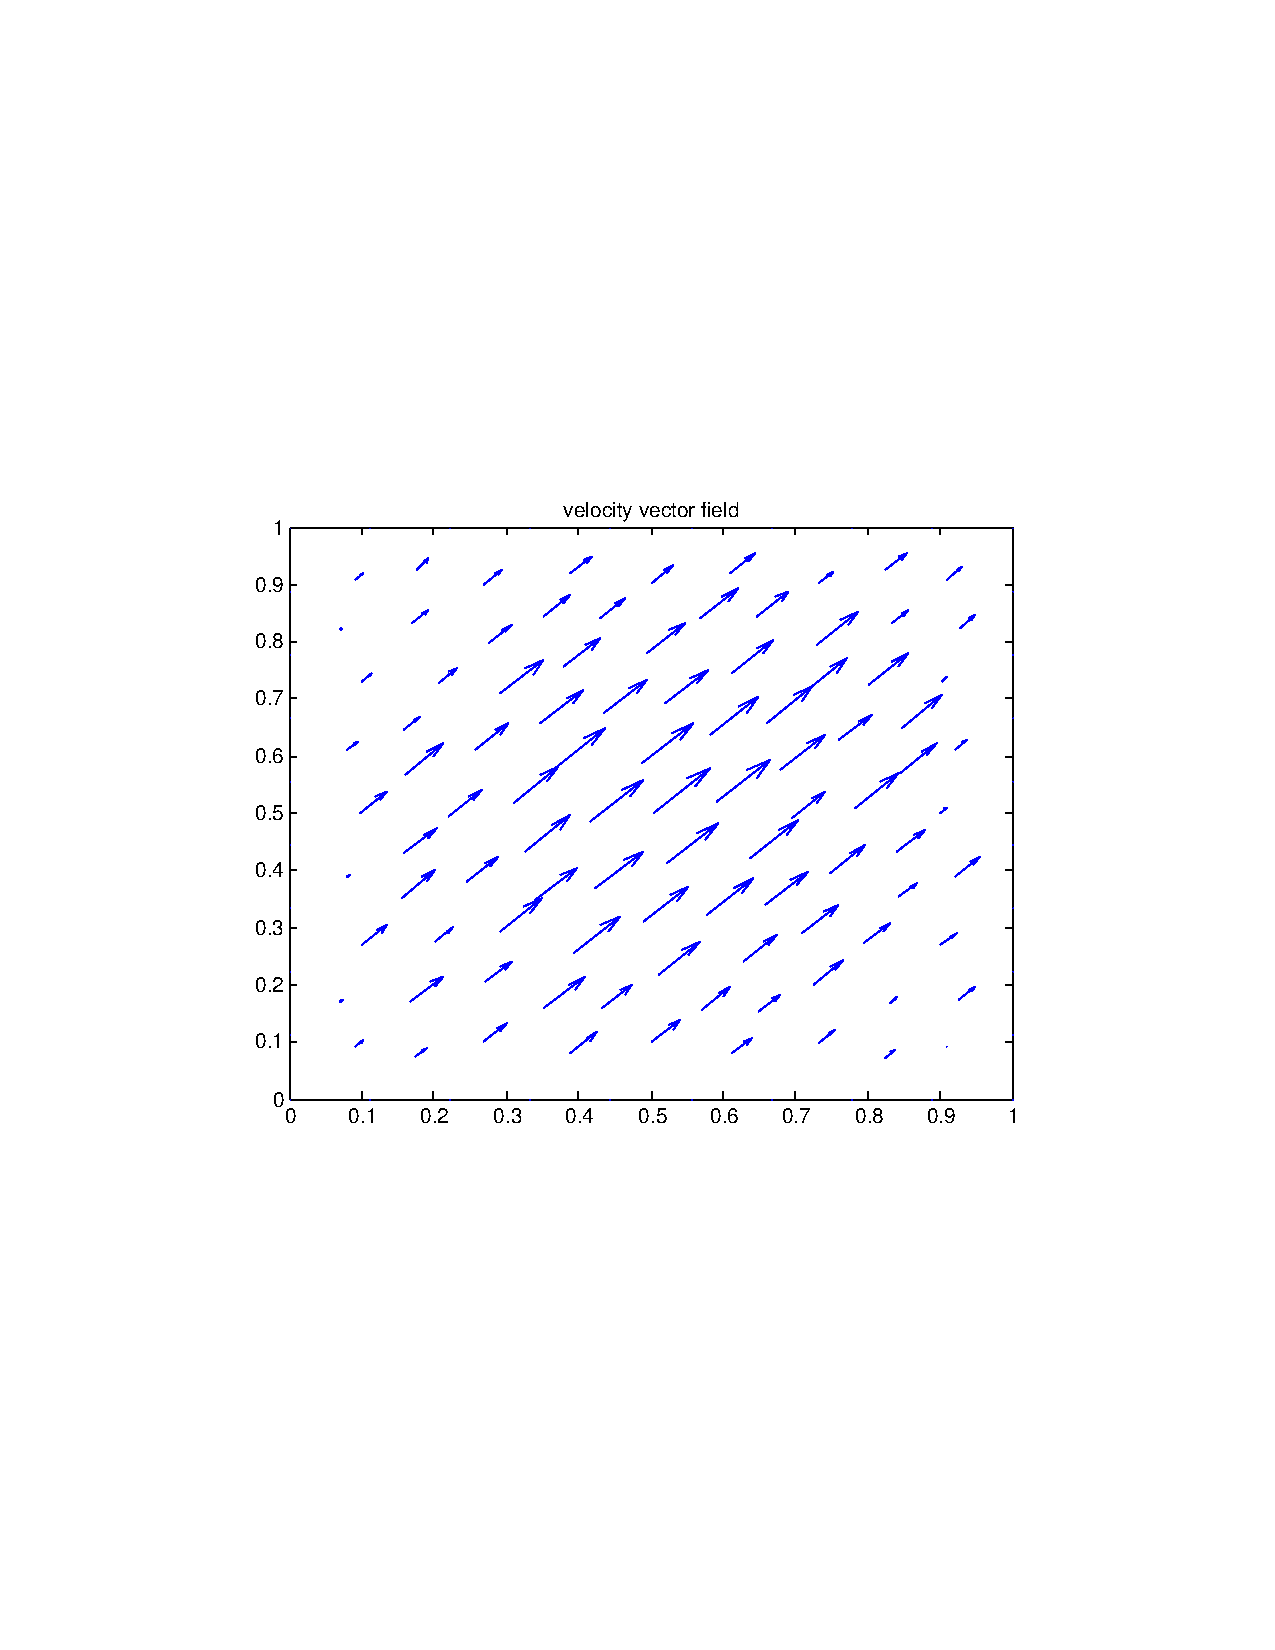
\includegraphics[scale=0.50]{./../files/box/1q.pdf}
                \caption{Velocity Field for $h = 0.1$}
            \end{center}
            \end{figure}

                \begin{figure}[htb]
                    \begin{center}
                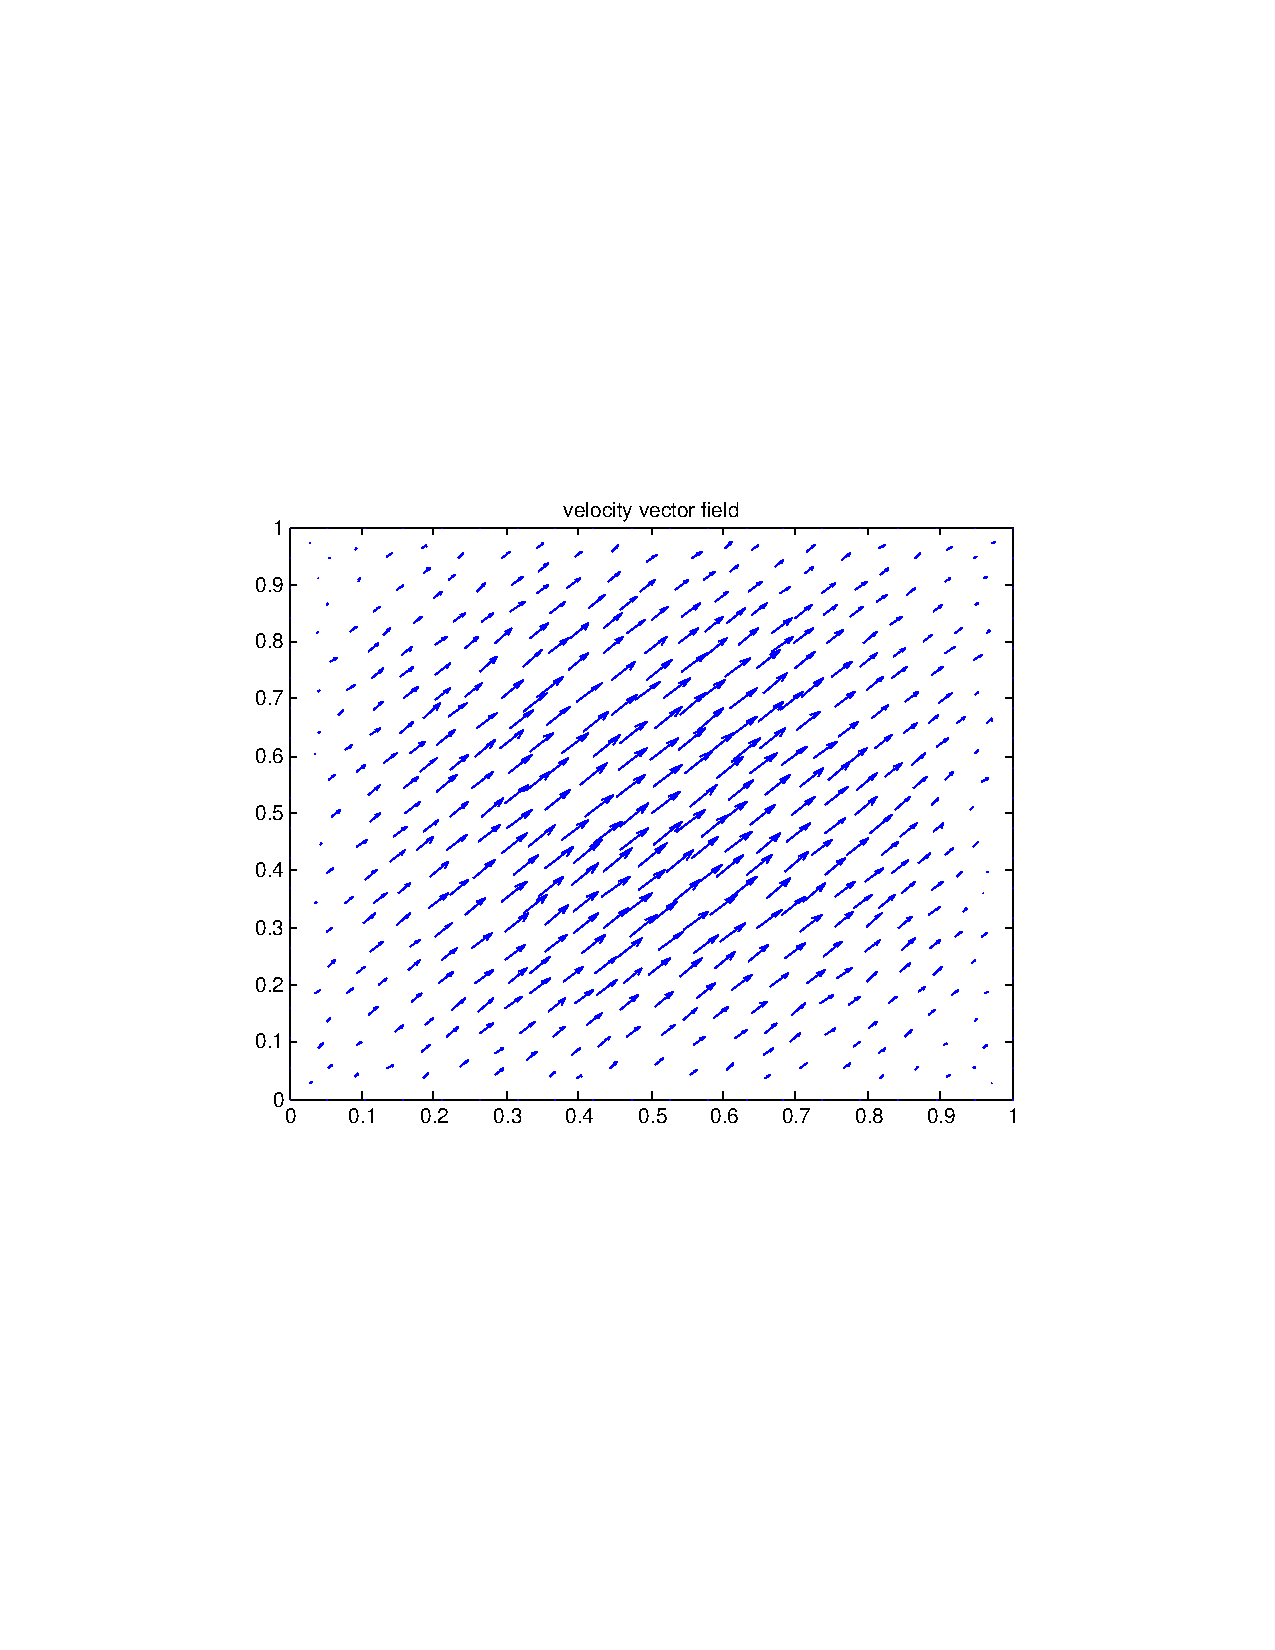
\includegraphics[scale=0.50]{./../files/box/2q.pdf}
                \caption{Velocity Field for $h = 0.05$}
            \end{center}
            \end{figure}

                \begin{figure}[htb]
                    \begin{center}
                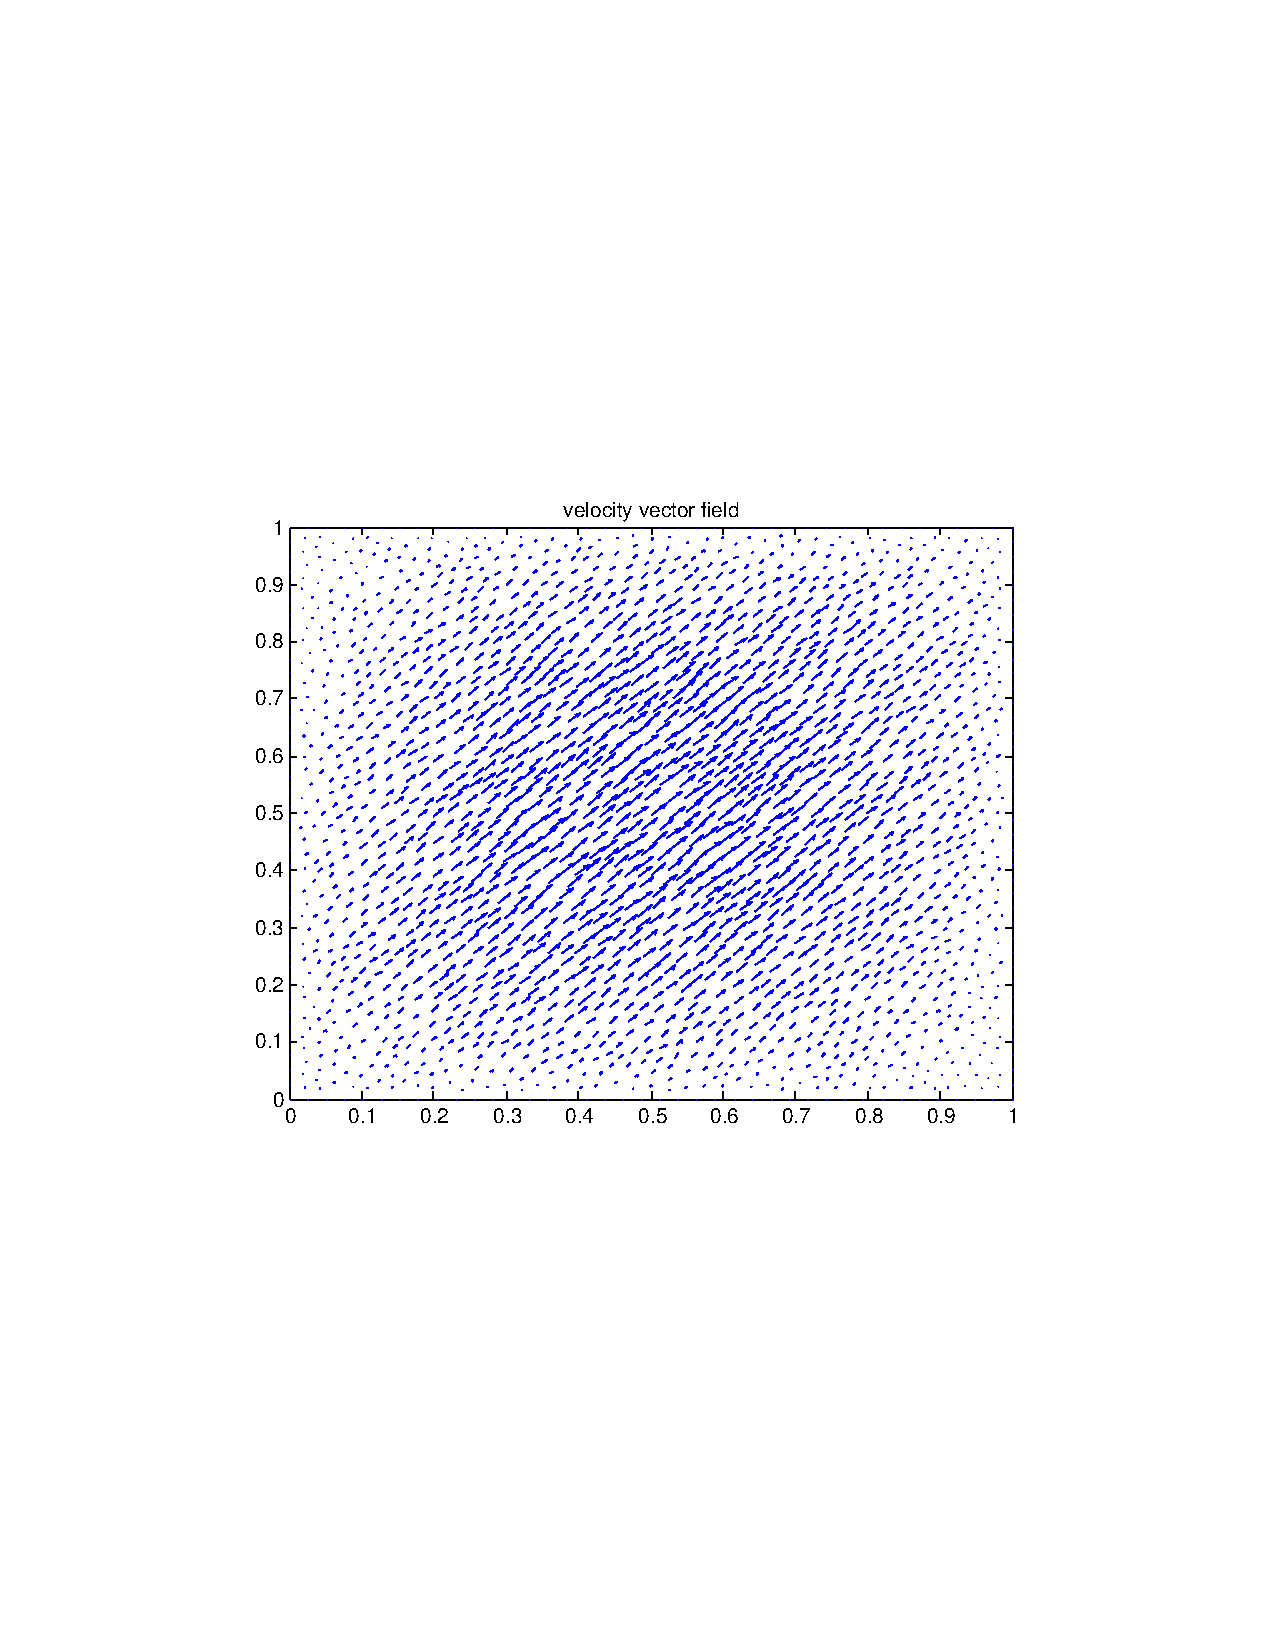
\includegraphics[scale=0.50]{./../files/box/3q.pdf}
                \caption{Velocity Field for $h = 0.025$}
            \end{center}
            \end{figure}

                \begin{figure}[htb]
                    \begin{center}
                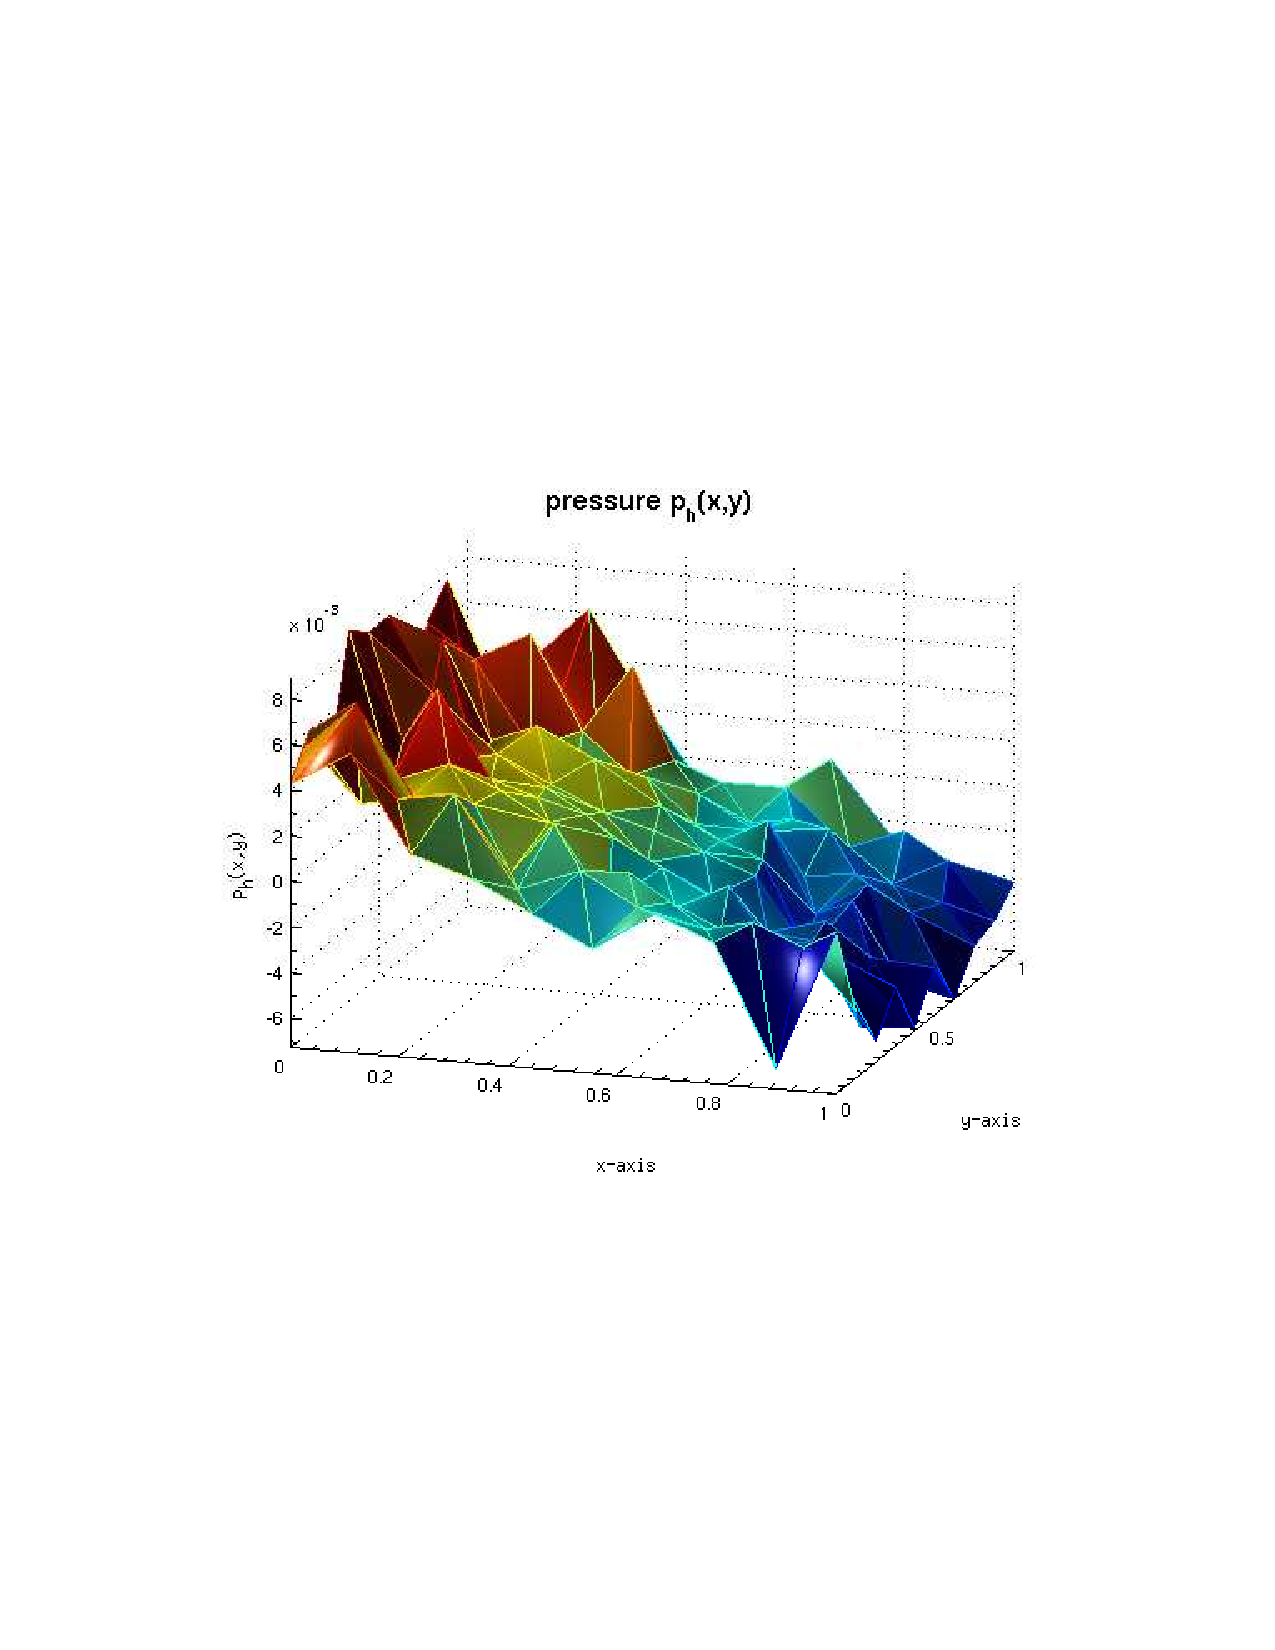
\includegraphics[scale=0.50]{./../files/box/1p.pdf}
                \caption{$p_h(x,y)$ for $h = 0.1$}
            \end{center}
            \end{figure}

                \begin{figure}[htb]
                    \begin{center}
                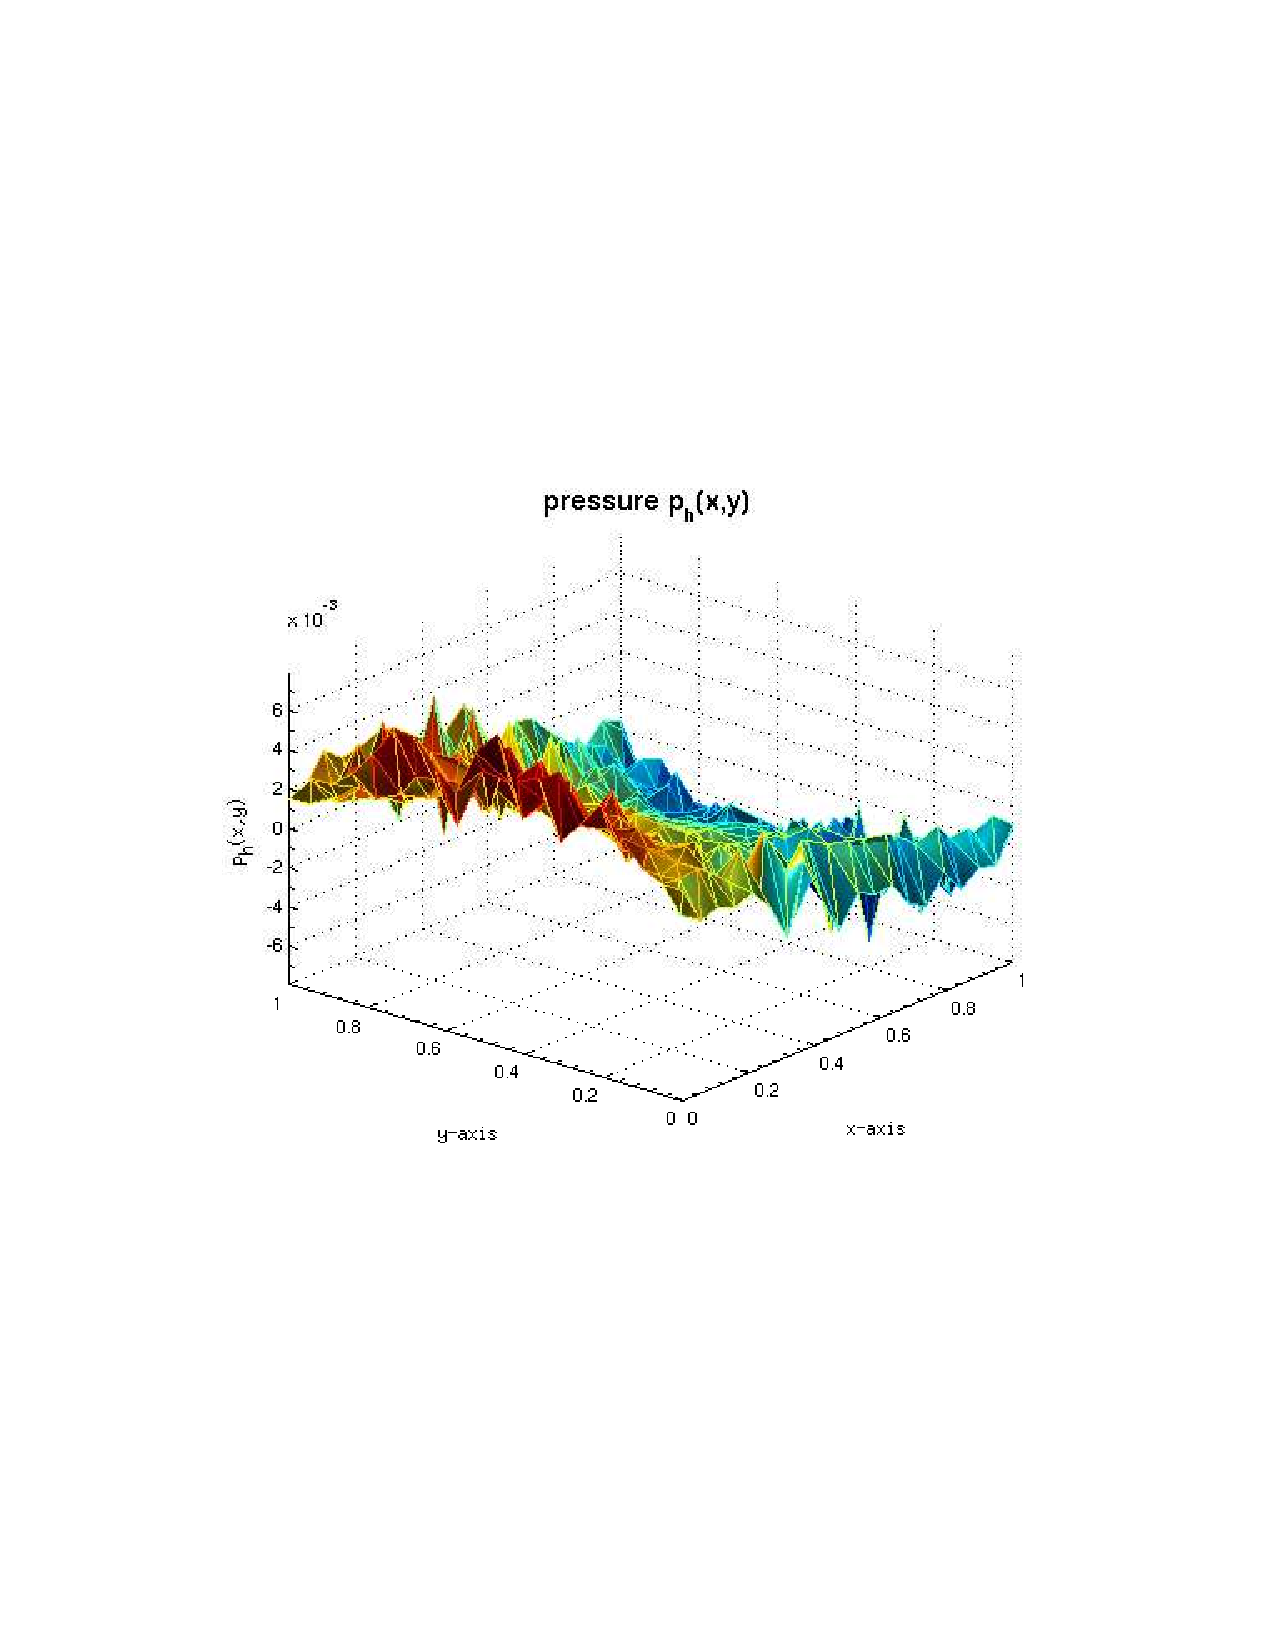
\includegraphics[scale=0.50]{./../files/box/3p.pdf}
                \caption{$p_h(x,y)$ for $h = 0.05$}
            \end{center}
            \end{figure}

                \begin{figure}[htb]
                    \begin{center}
                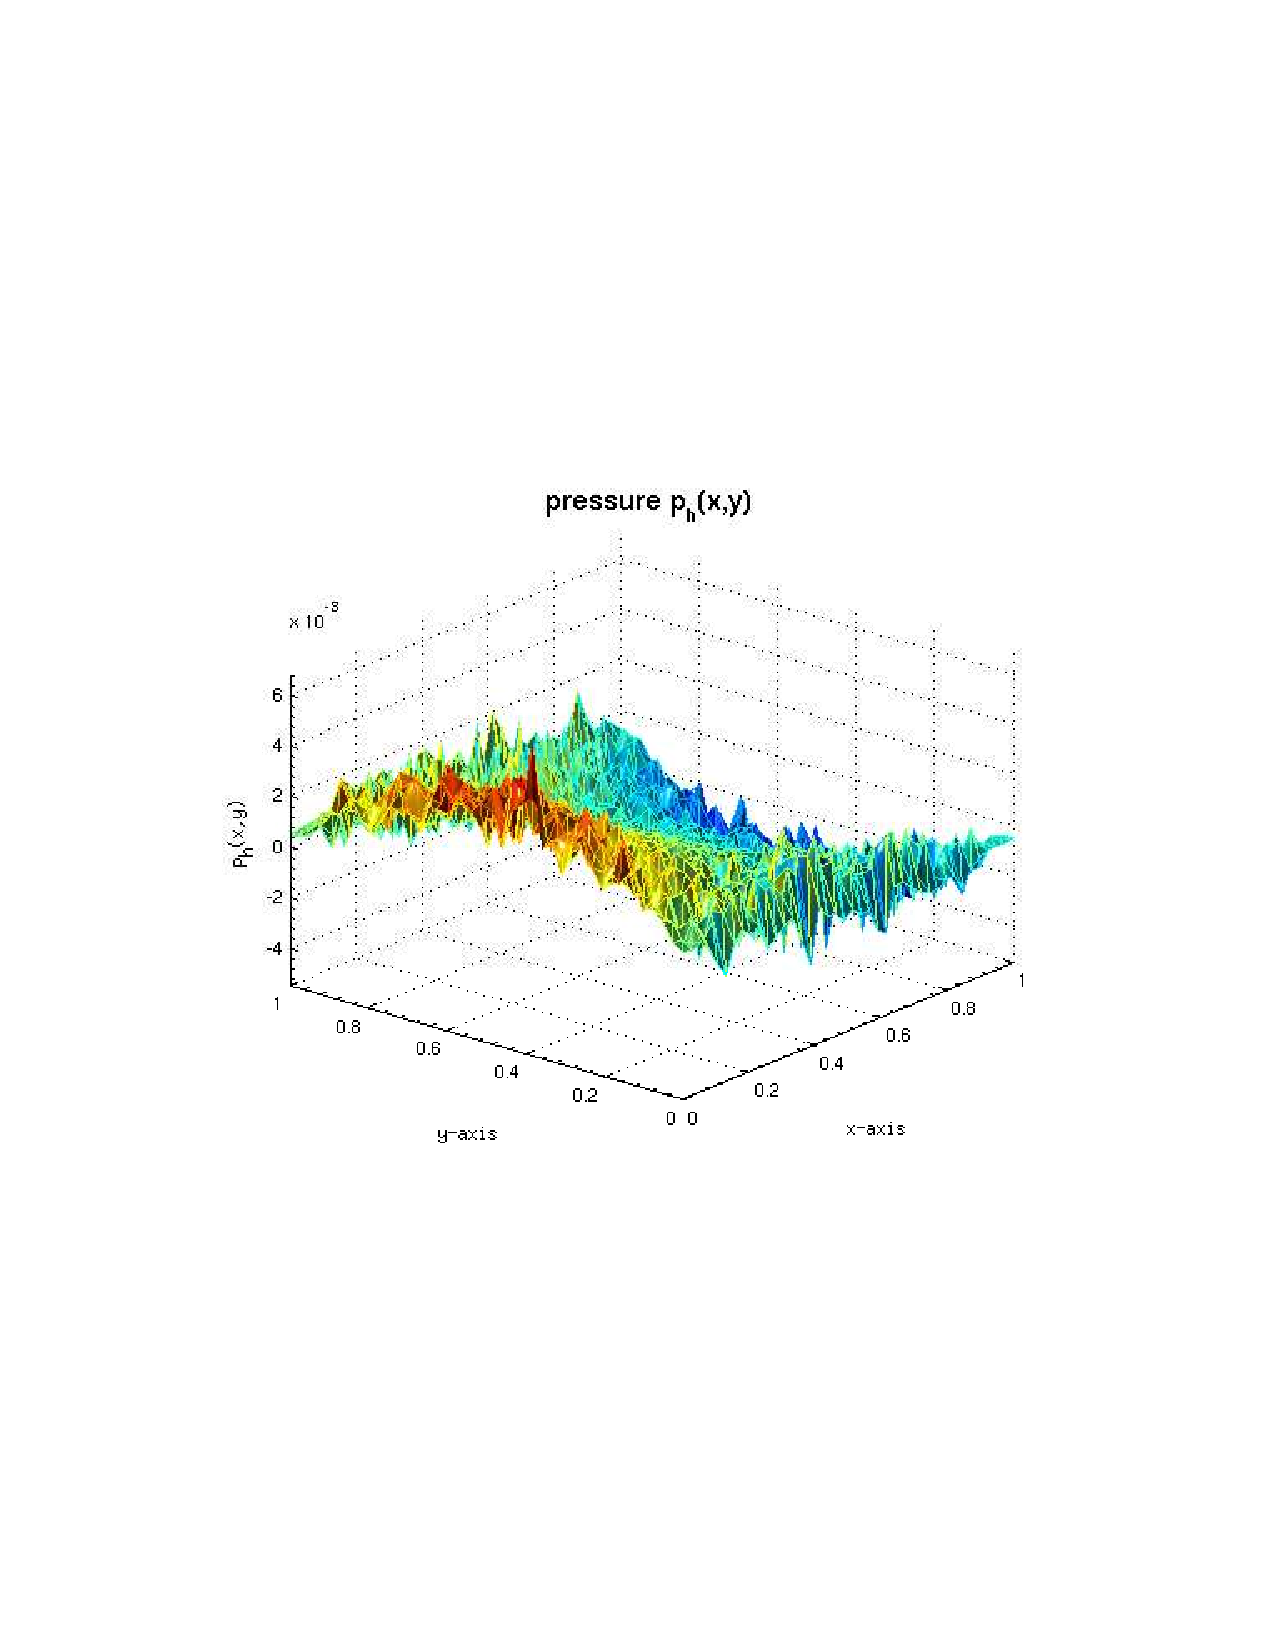
\includegraphics[scale=0.50]{./../files/box/2p.pdf}
                \caption{$p_h(x,y)$ for $h = 0.025$}
            \end{center}
            \end{figure}

                \begin{figure}[htb]
                    \begin{center}
                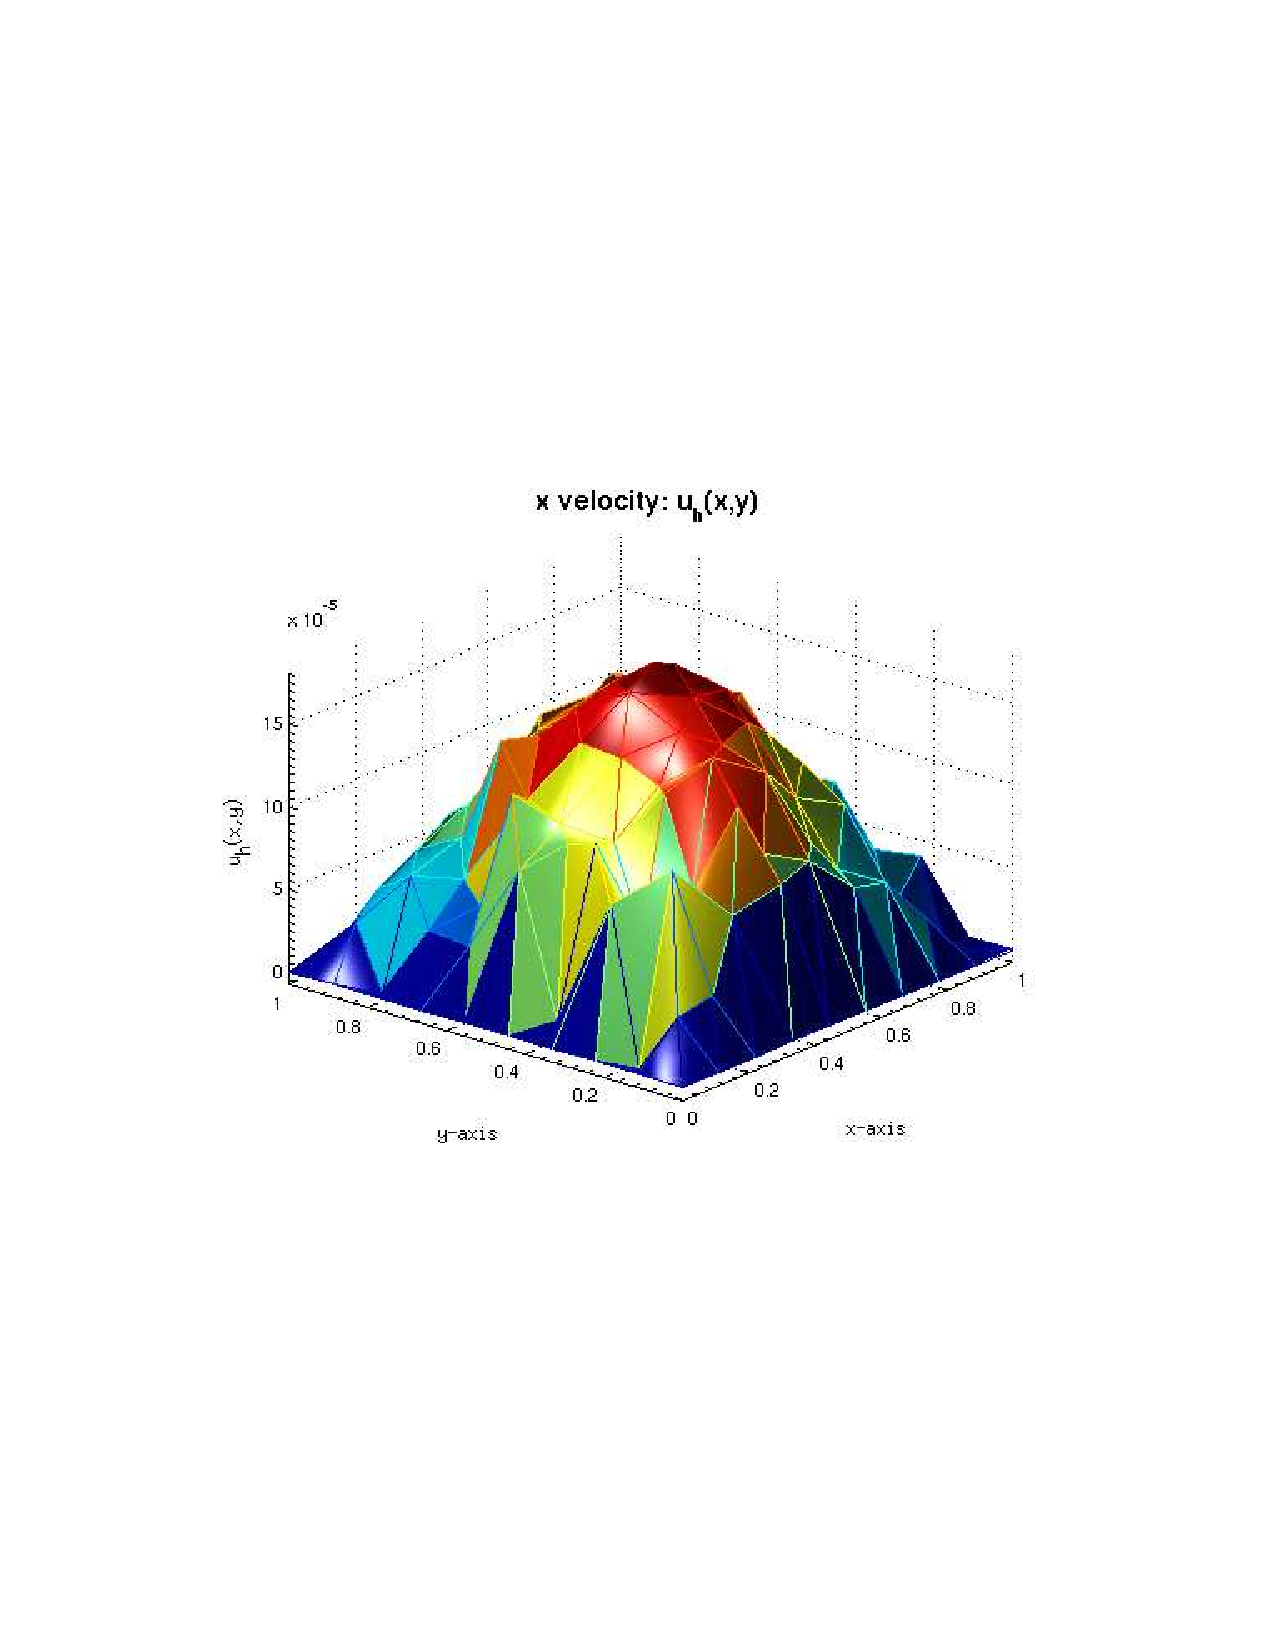
\includegraphics[scale=0.50]{./../files/box/1u.pdf}
                \caption{$u_h(x,y)$ for $h = 0.1$}
            \end{center}
            \end{figure}

                \begin{figure}[htb]
                    \begin{center}
                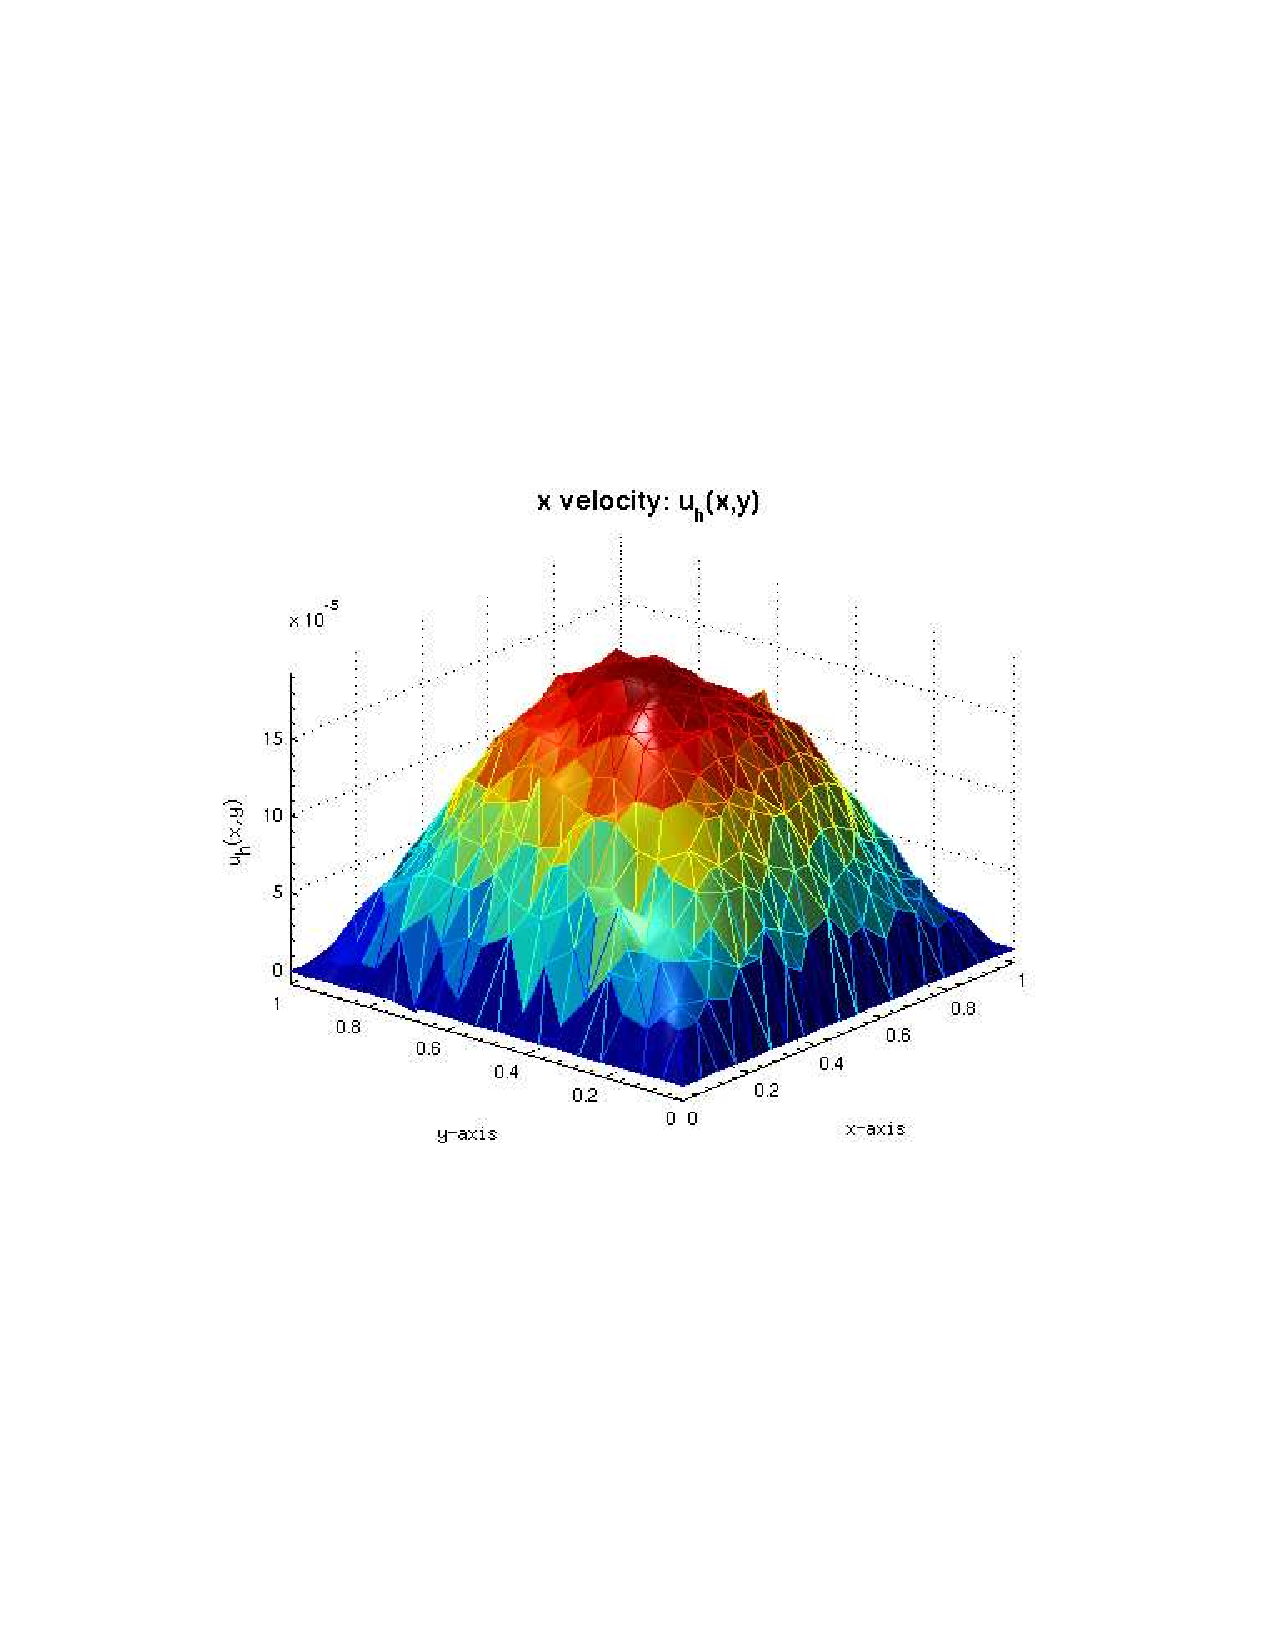
\includegraphics[scale=0.50]{./../files/box/2u.pdf}
                \caption{$u_h(x,y)$ for $h = 0.05$}
            \end{center}
            \end{figure}

                \begin{figure}[htb]
                    \begin{center}
                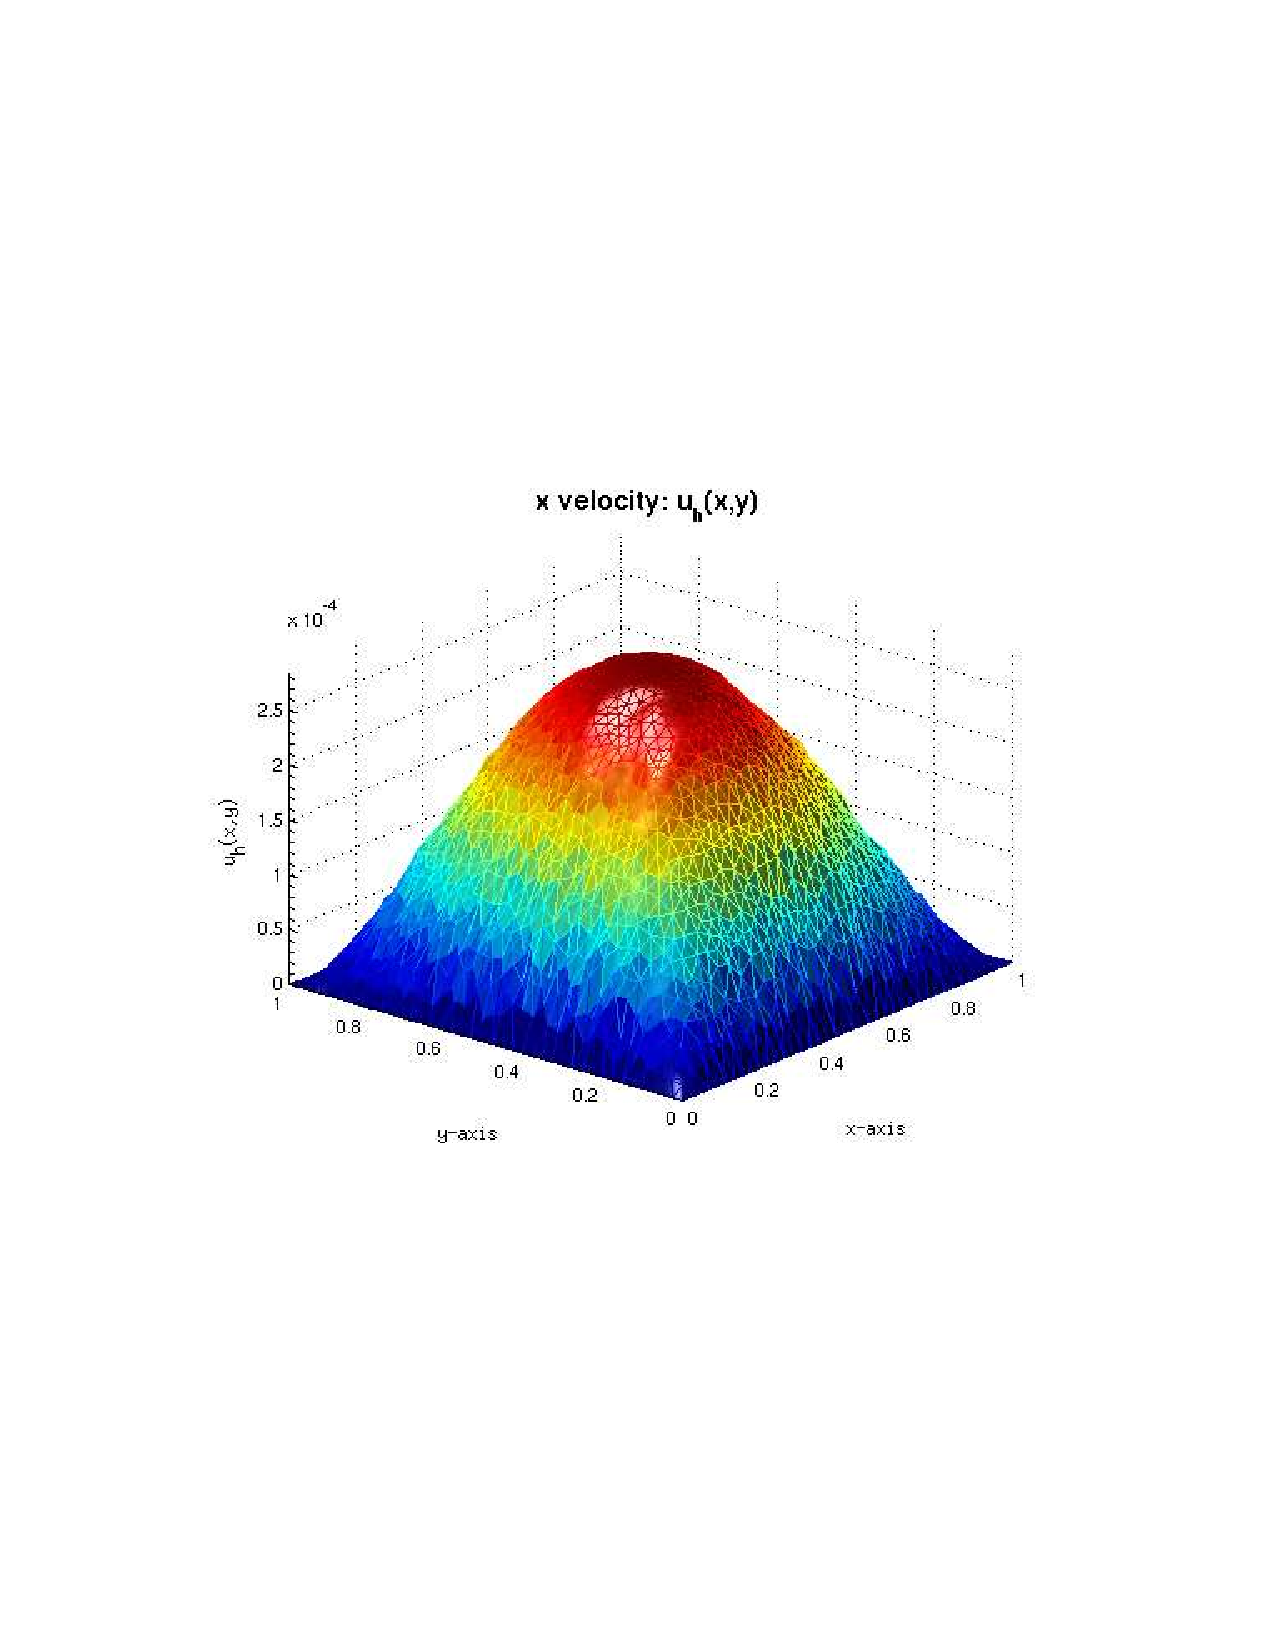
\includegraphics[scale=0.50]{./../files/box/3u.pdf}
                \caption{$u_h(x,y)$ for $h = 0.025$}
            \end{center}
            \end{figure}
                \begin{figure}[htb]
                    \begin{center}
                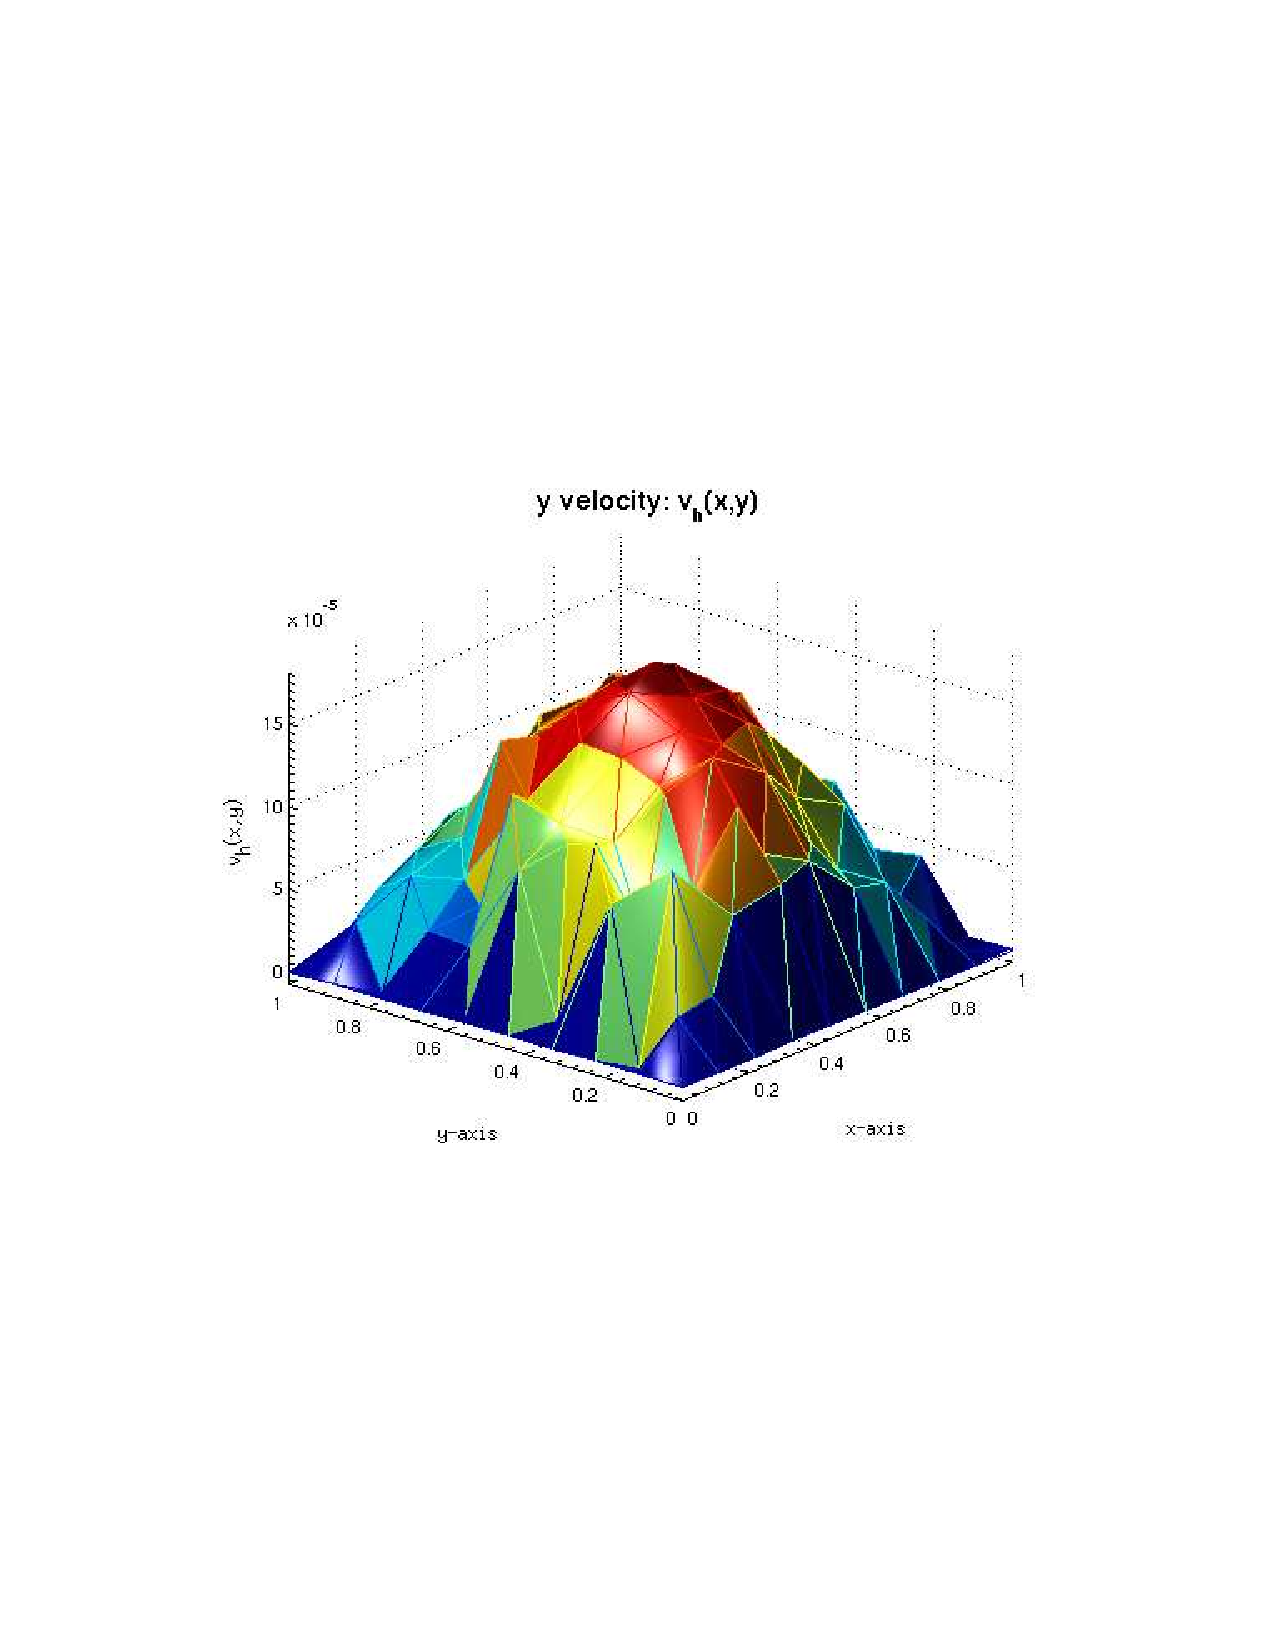
\includegraphics[scale=0.50]{./../files/box/1v.pdf}
                \caption{$v_h(x,y)$ for $h = 0.1$}
            \end{center}
            \end{figure}

                \begin{figure}[htb]
                    \begin{center}
                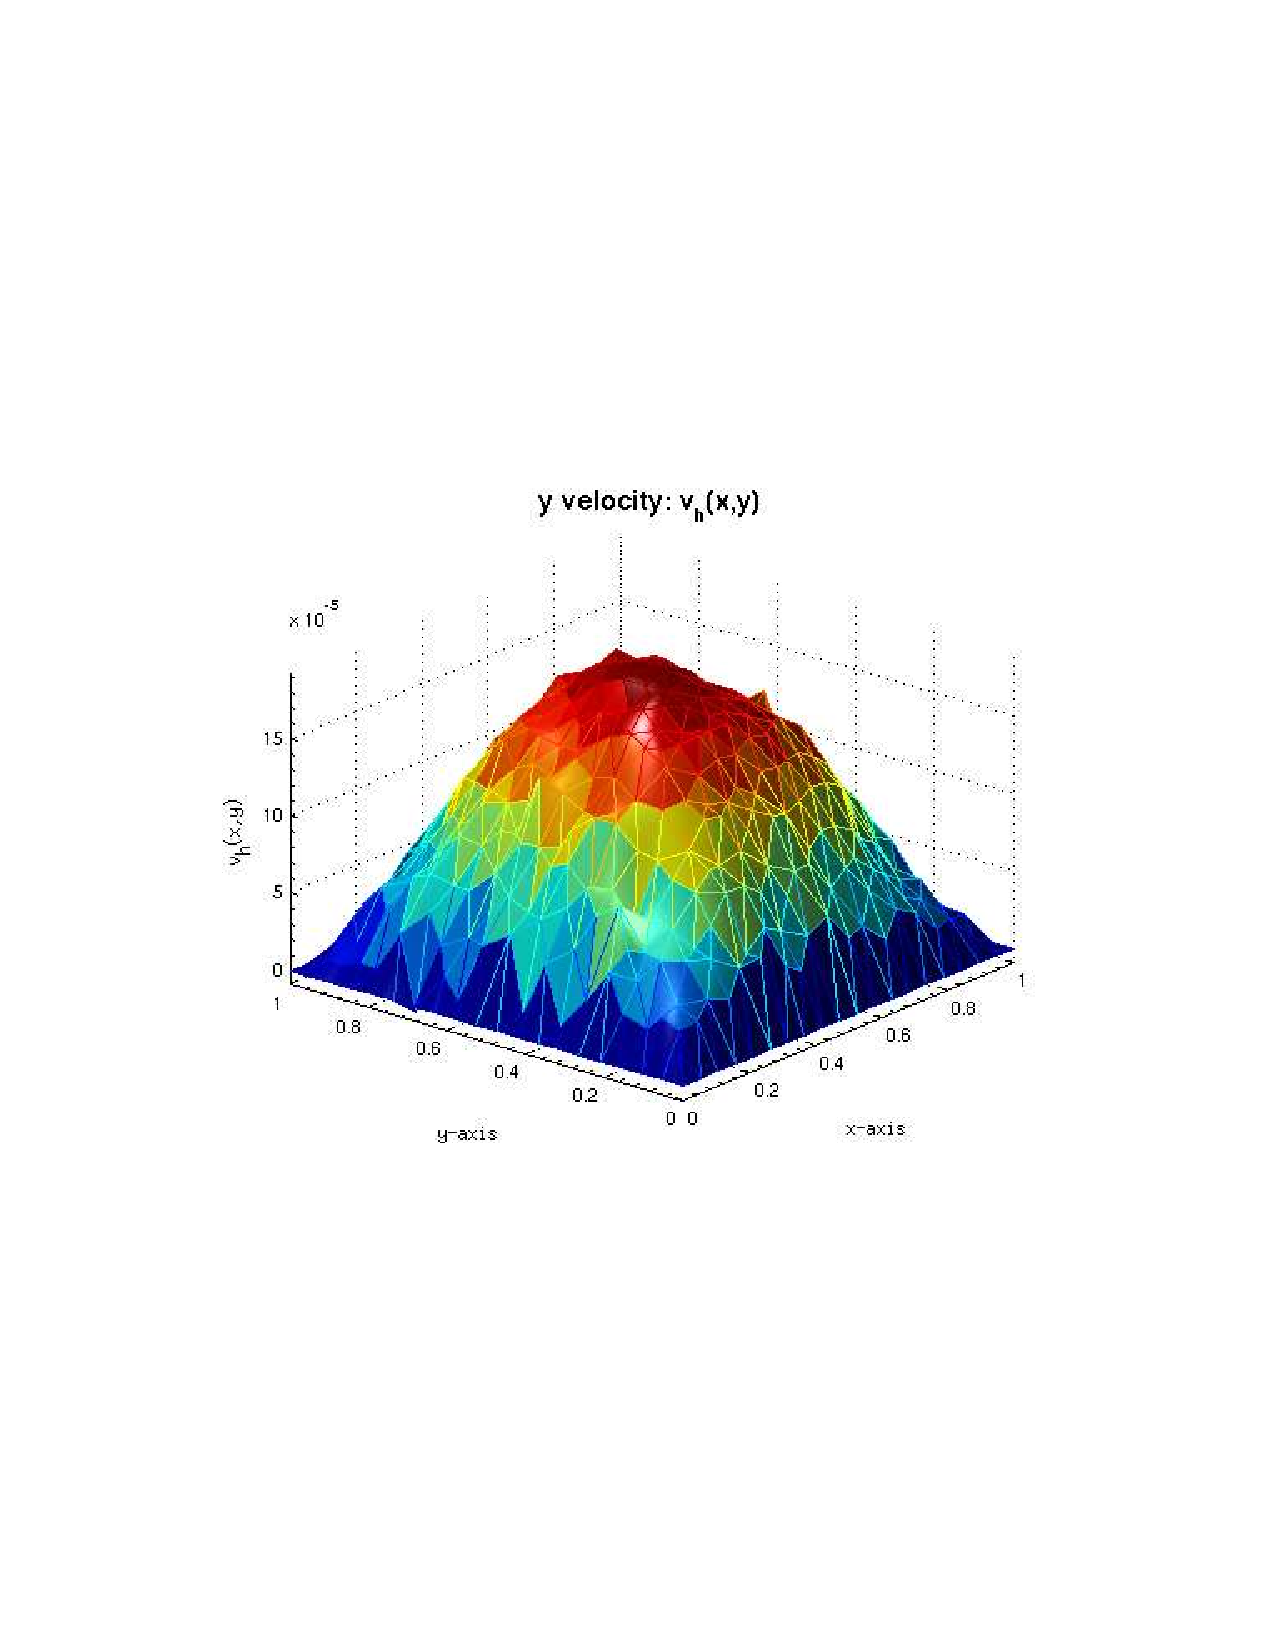
\includegraphics[scale=0.50]{./../files/box/2v.pdf}
                \caption{$v_h(x,y)$ for $h = 0.05$}
            \end{center}
            \end{figure}

                \begin{figure}[htb]
                    \begin{center}
                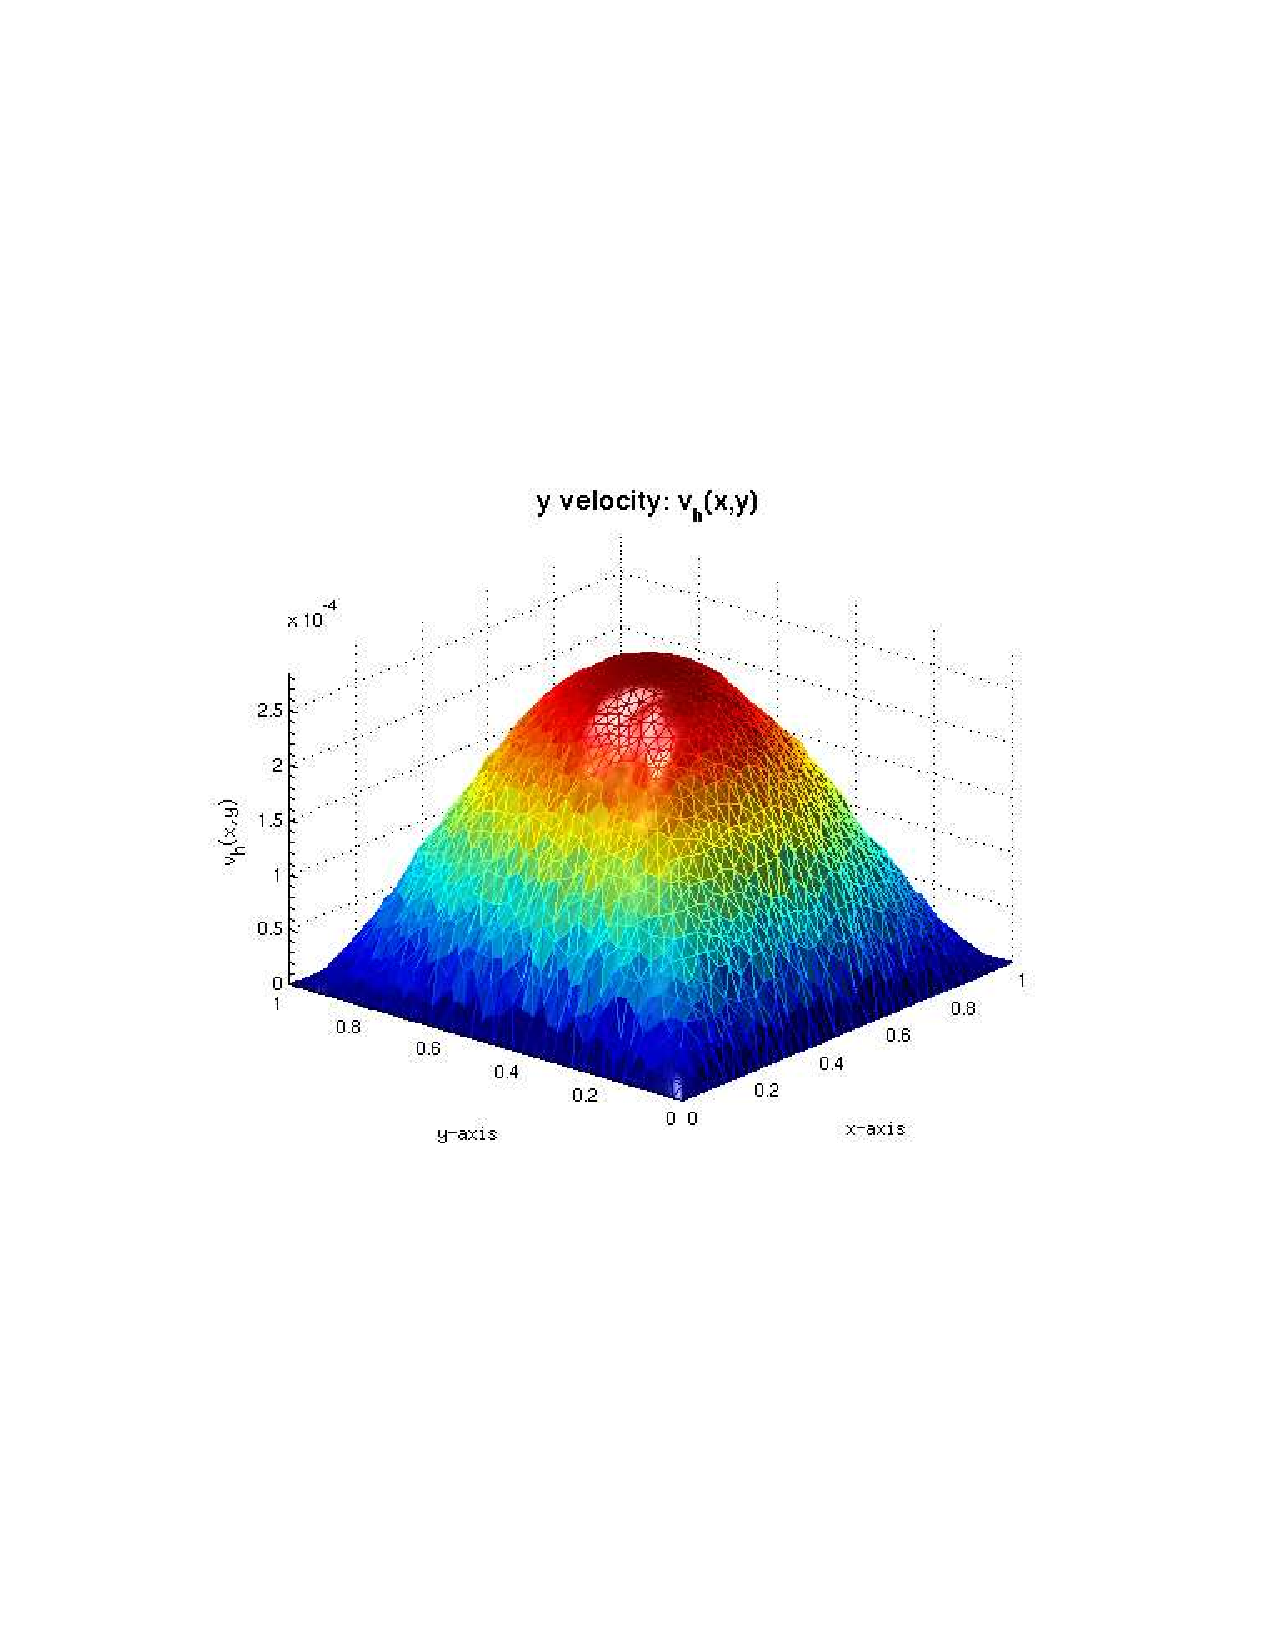
\includegraphics[scale=0.50]{./../files/box/3v.pdf}
                \caption{$v_h(x,y)$ for $h = 0.025$}
            \end{center}
            \end{figure}


            The velocity functions \textit{seem} to converge to nice, smooth solutions. Again, as I have nothing to compare
            it against, I cannot say for certain. The solution makes sense as it is forming a ``bubble'' to deal with the pressure
            in the system while still maintaining zero boundary conditions, similar to it having some factor of $\sin(\pi x) \sin(\pi y)$ in both
            $u(x,y)$ and $v(x,y)$.

            The pressure coefficients are found by substituting back into the perturbed system. Since the system corresponding to those values was the
            culprit for making our system poorly conditioned, it makes sense that the coefficients seem oscillatory. By employing the very rigorous process of
            ``eyeball integration'' (a.k.a looking at the plot), it would appear from observing the symmetry that the mean-zero condition has been satisfied.

            It should be noted that even though the velocity basis functions were quadratic and so are defined on 6 nodes of each triangle, for sake
            of plotting the data, the coefficients were downgraded to a linear representation. This was also at the suggestion of Dr. Borggaard when I inquired
            about plotting methods for higher order elements.

            \clearpage
            \subsection{Other Geometries}

            I will now present other plots with novel geometries. All meshes had characteristic length $h = 0.025$.

            The forcing function for was $\vect{f}(x,y) = 1\text{e}-2 (y, -x)$ for this first set of plots.

                \begin{figure}[htb]
                    \begin{center}
                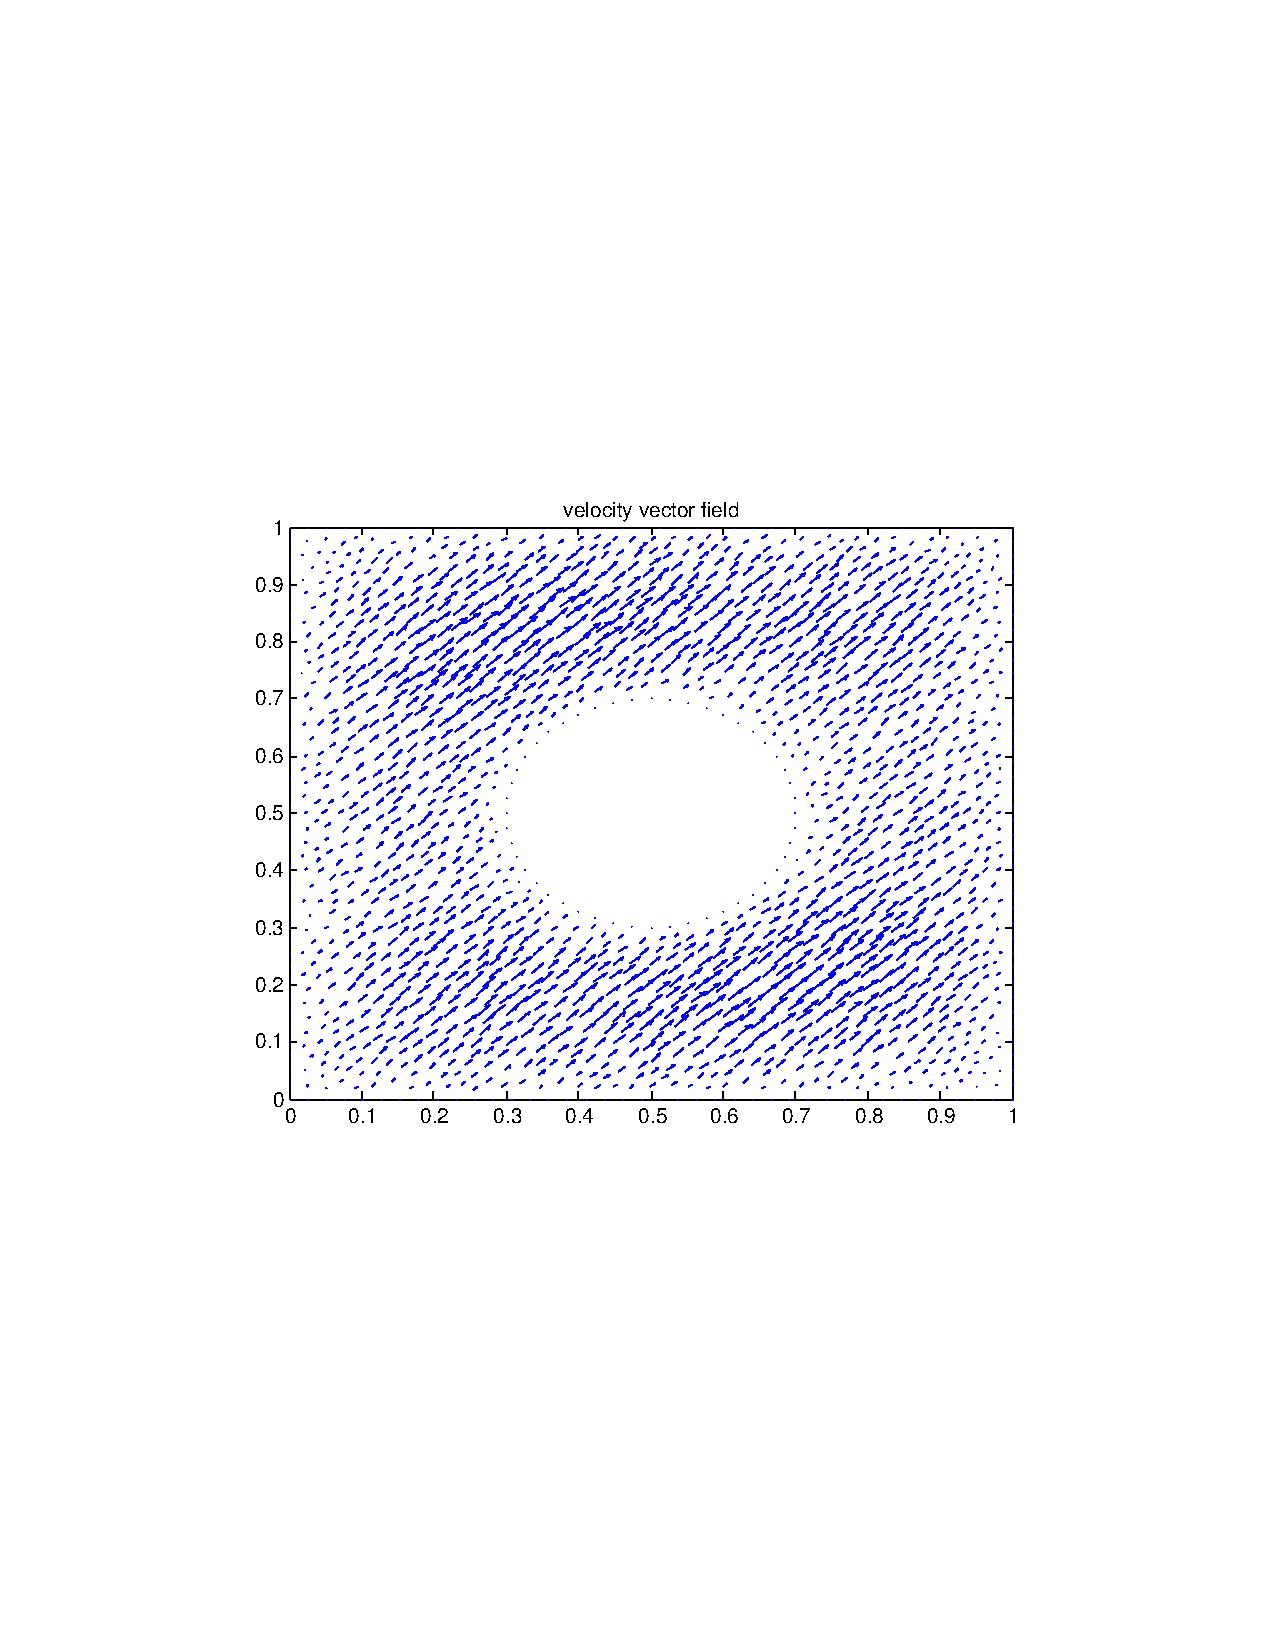
\includegraphics[scale=0.50]{./../files/box-circle/q.pdf}
                \caption{Velocity Field  for $h = 0.025$}
            \end{center}
            \end{figure}
                \begin{figure}[htb]
                    \begin{center}
                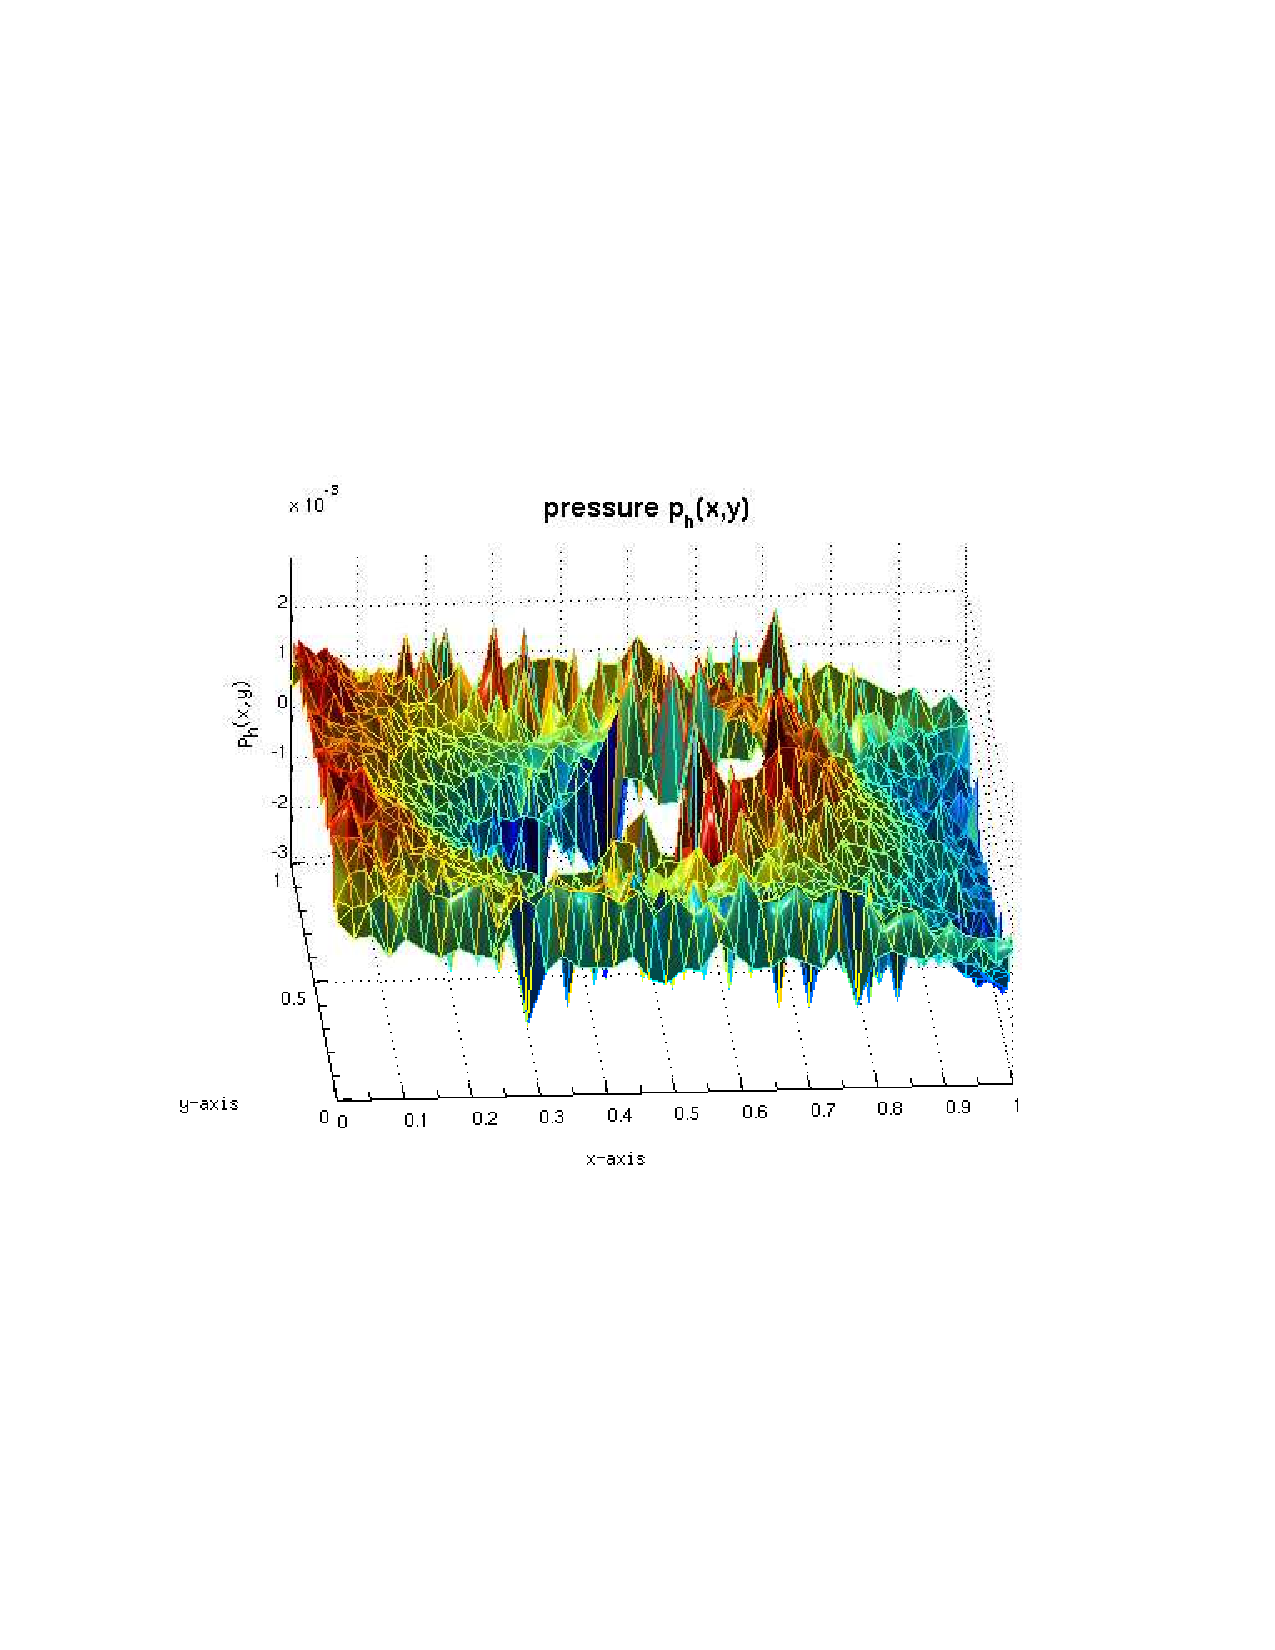
\includegraphics[scale=0.50]{./../files/box-circle/p.pdf}
                \caption{$p_h(x,y)$ for $h = 0.025$}
            \end{center}
            \end{figure}

                \begin{figure}[htb]
                    \begin{center}
                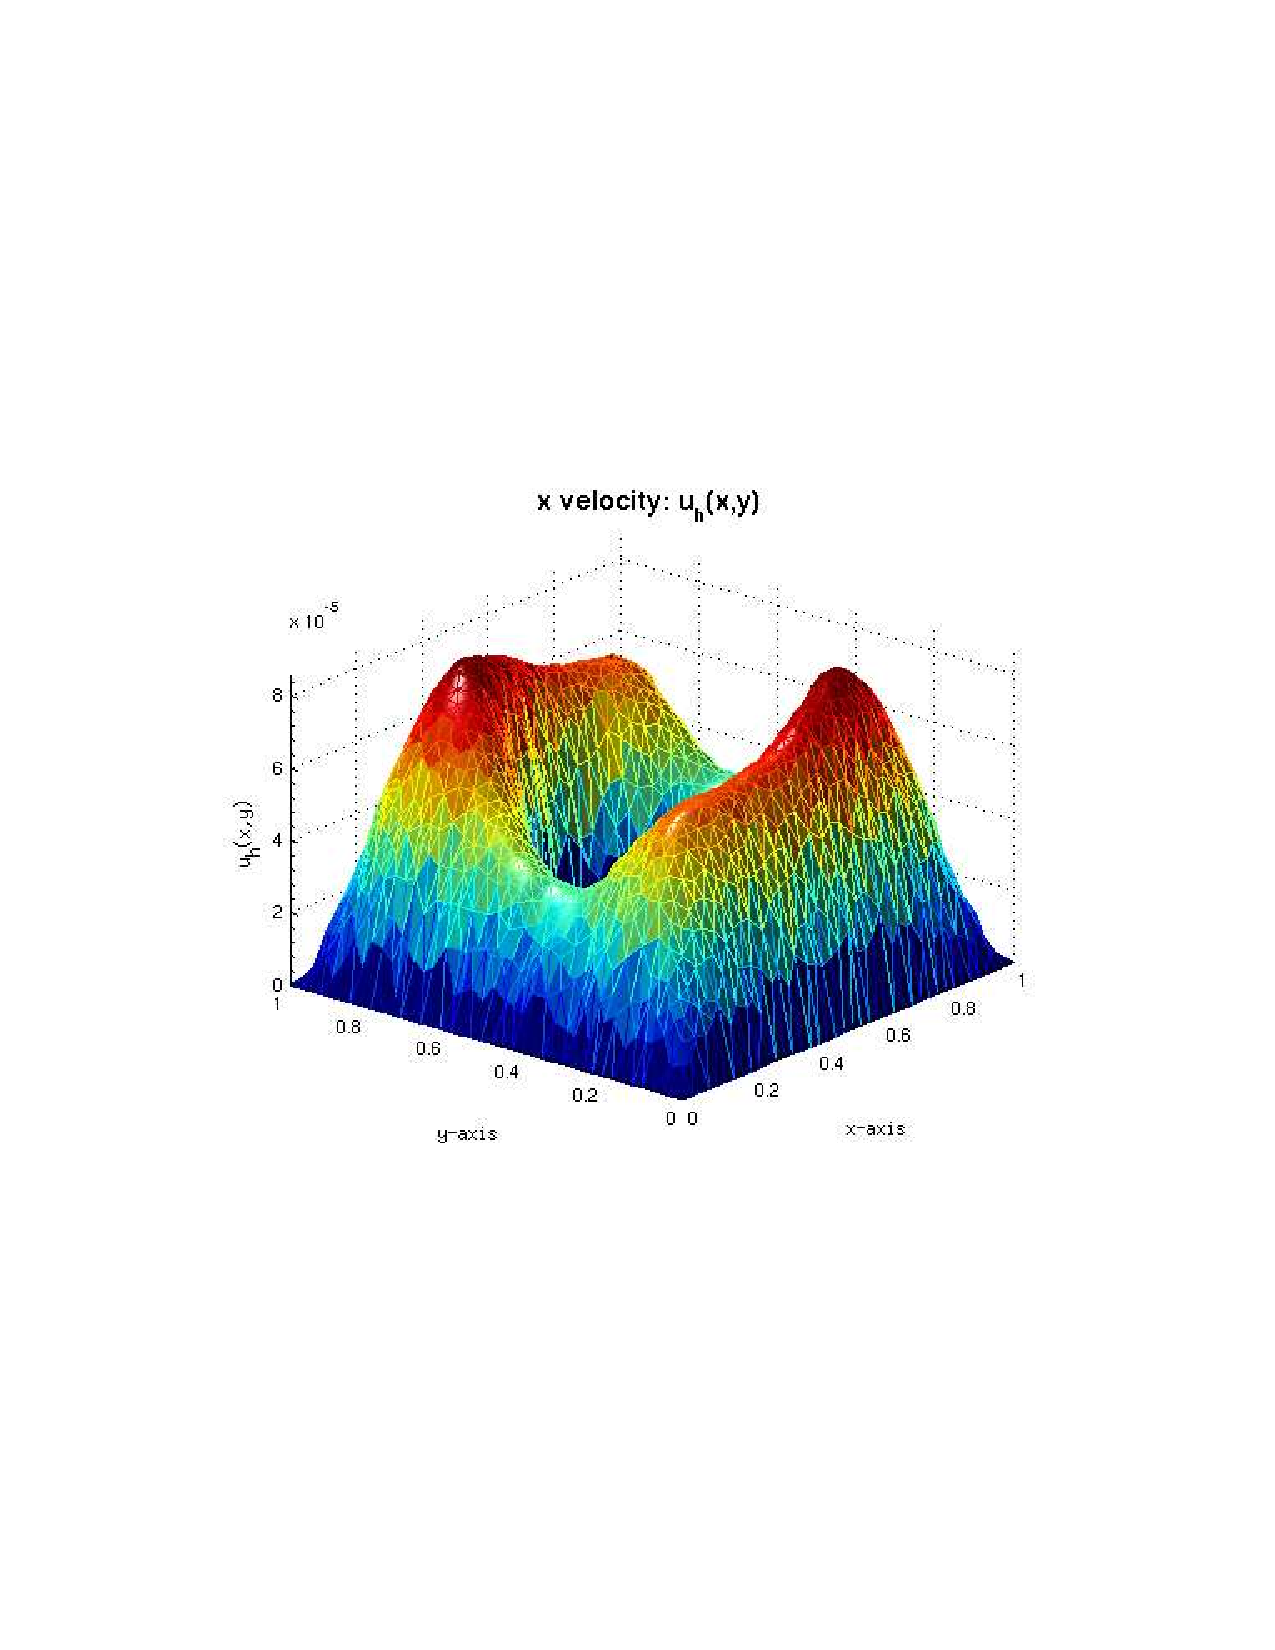
\includegraphics[scale=0.50]{./../files/box-circle/u.pdf}
                \caption{$u_h(x,y)$ for $h = 0.025$}
            \end{center}
            \end{figure}

                \begin{figure}[htb]
                    \begin{center}
                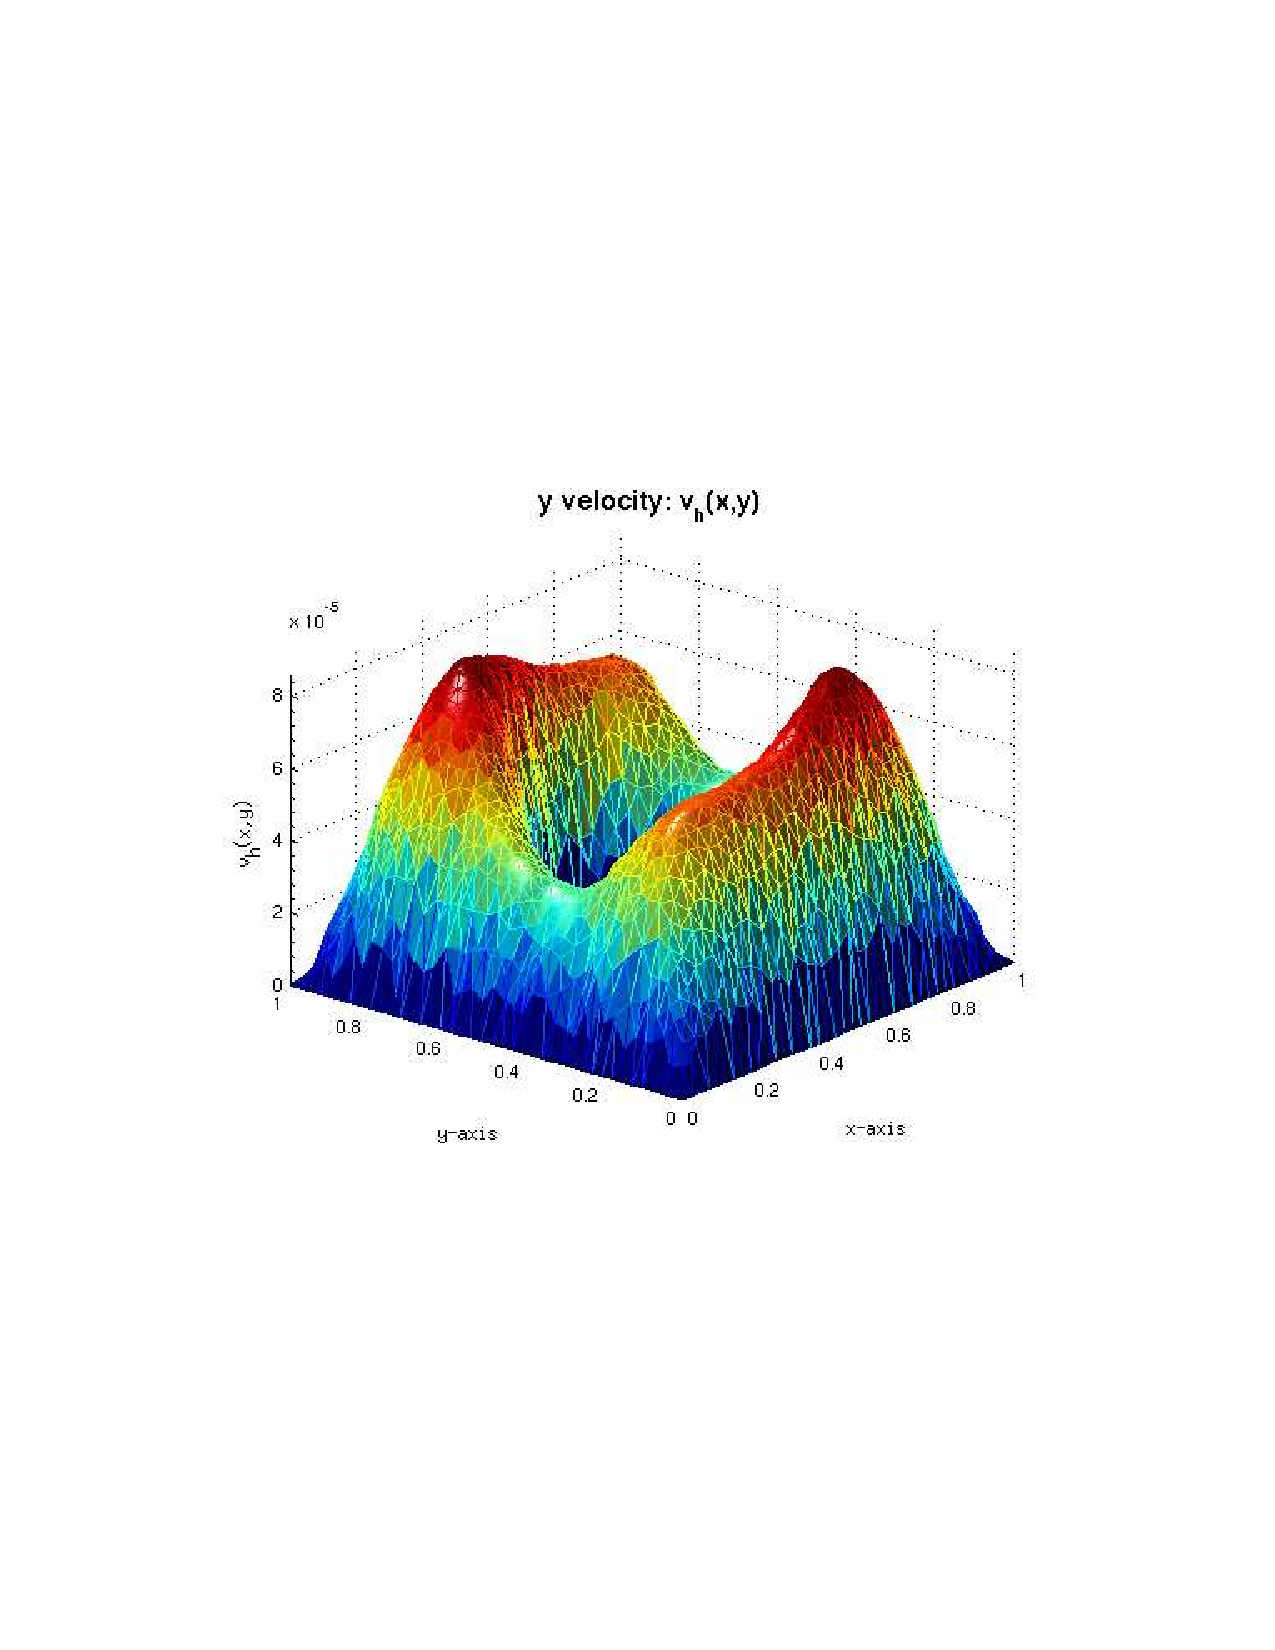
\includegraphics[scale=0.50]{./../files/box-circle/v.pdf}
                \caption{$v_h(x,y)$ for $h = 0.025$}
            \end{center}
            \end{figure}


            \clearpage

            And for this last set, the forcing function was $\vect{f}(x,y) =
            10 \cos(\pi x) y^3 - 4x, 0)$. This function was not chosen for any particular
            reason other than to be complicated.
                \begin{figure}[htb]
                    \begin{center}
                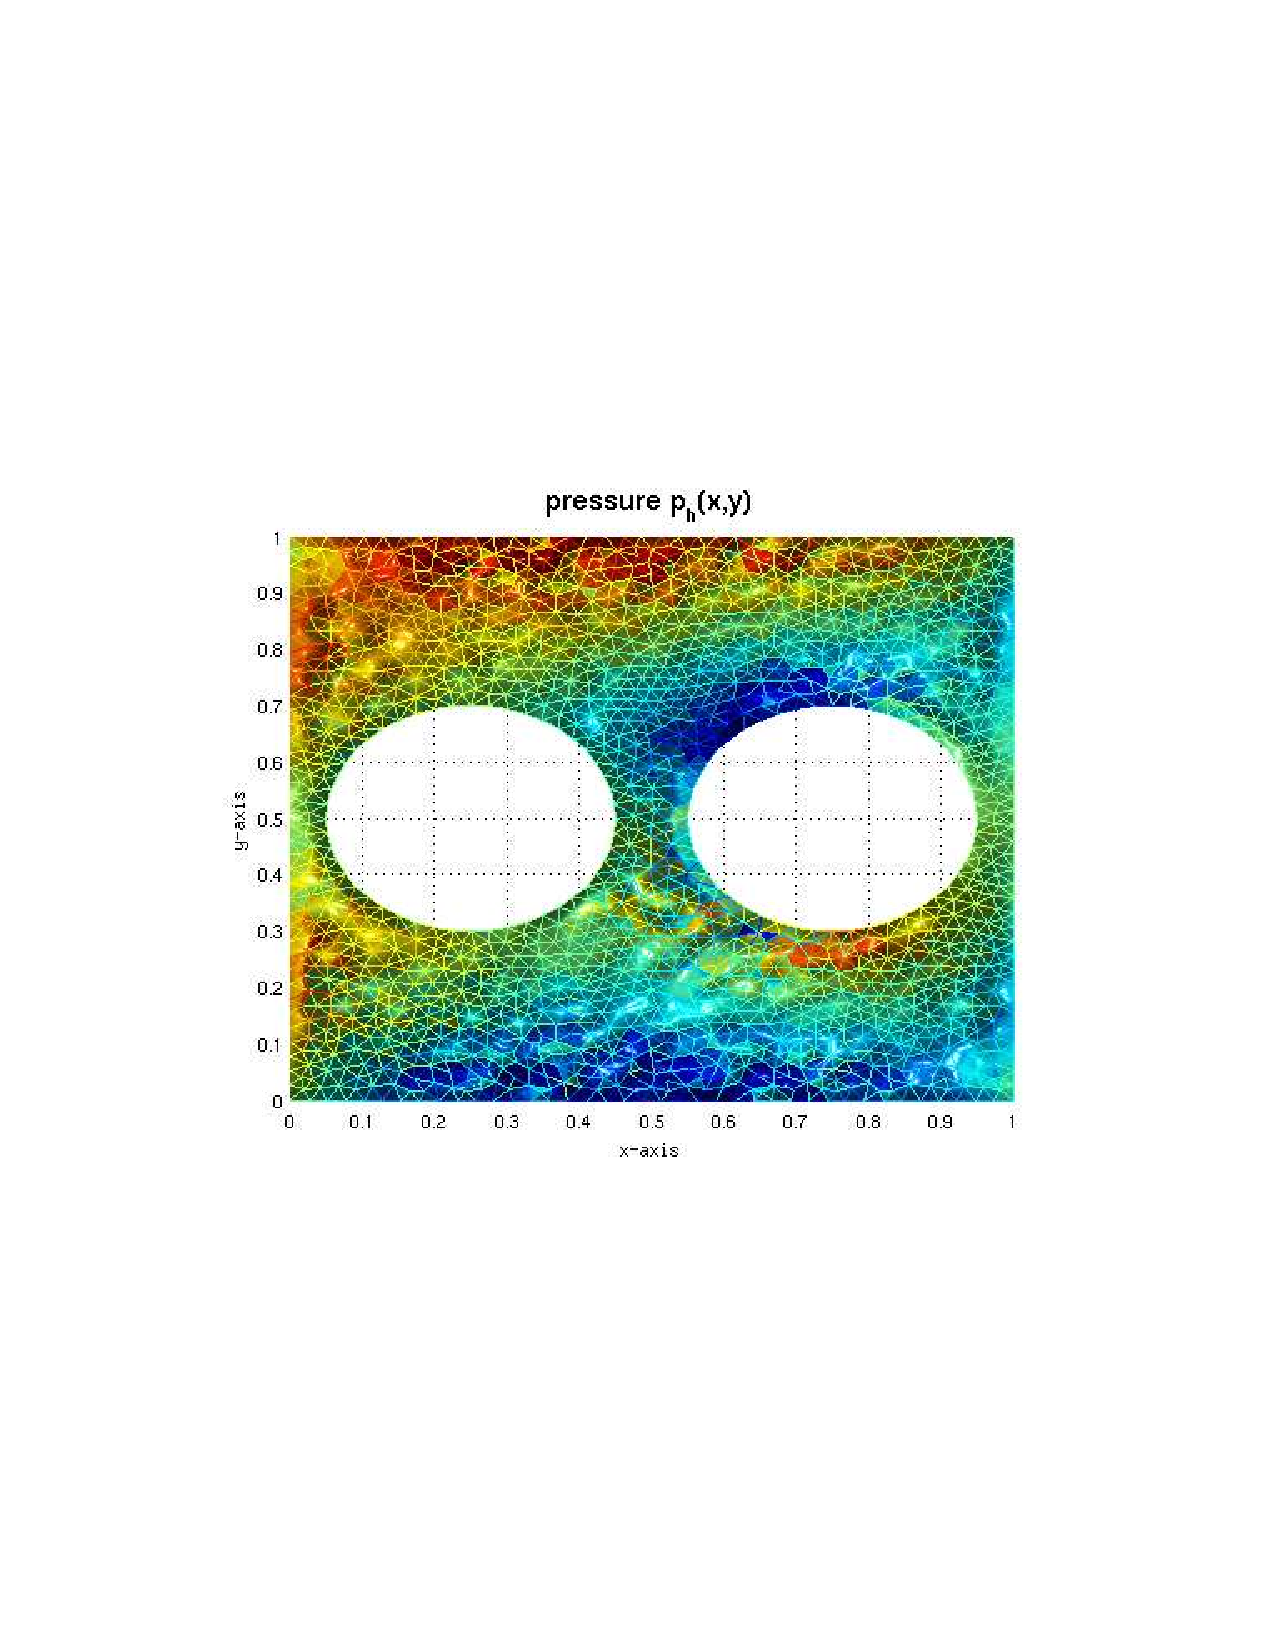
\includegraphics[scale=0.50]{./../files/crazy/p.pdf}
                \caption{$p_h(x,y)$ for $h = 0.025$}
            \end{center}
            \end{figure}

                \begin{figure}[htb]
                    \begin{center}
                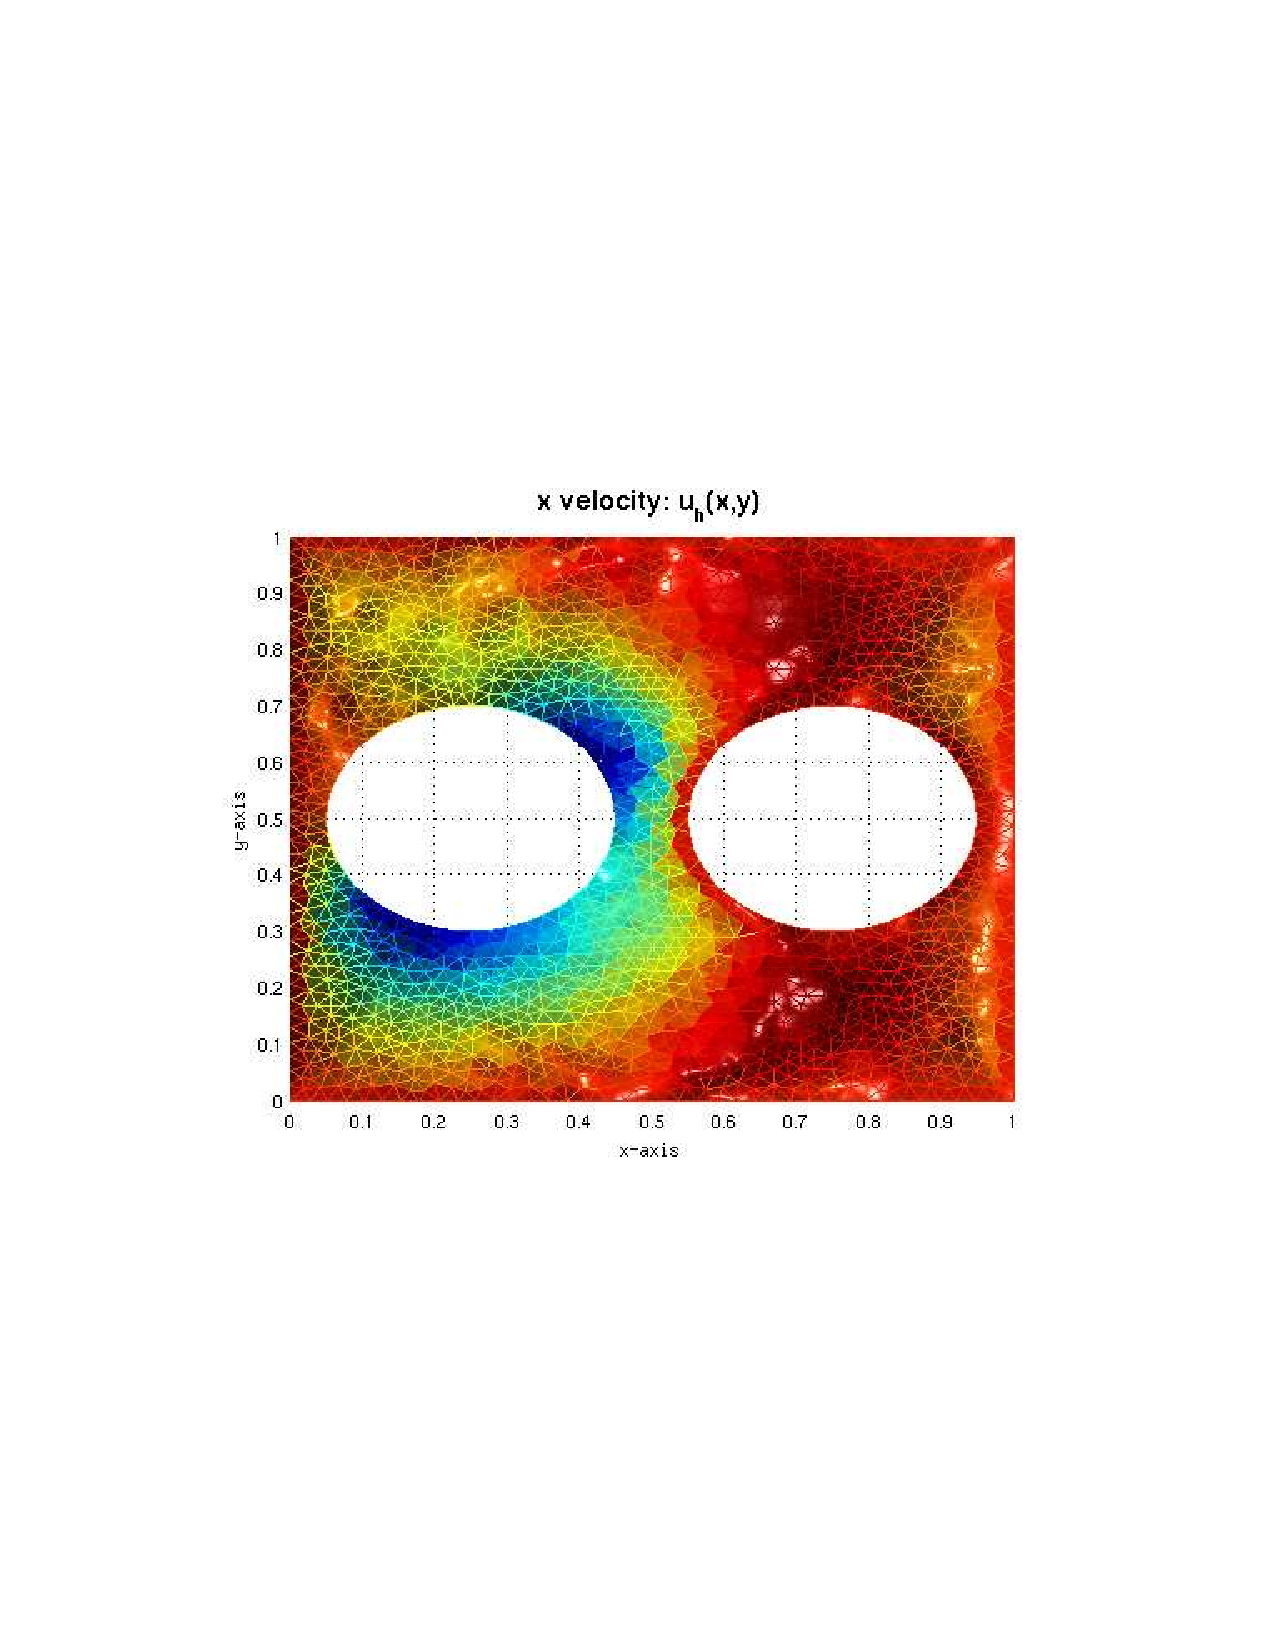
\includegraphics[scale=0.50]{./../files/crazy/u.pdf}
                \caption{$u_h(x,y)$ for $h = 0.025$}
            \end{center}
            \end{figure}

                \begin{figure}[htb]
                    \begin{center}
                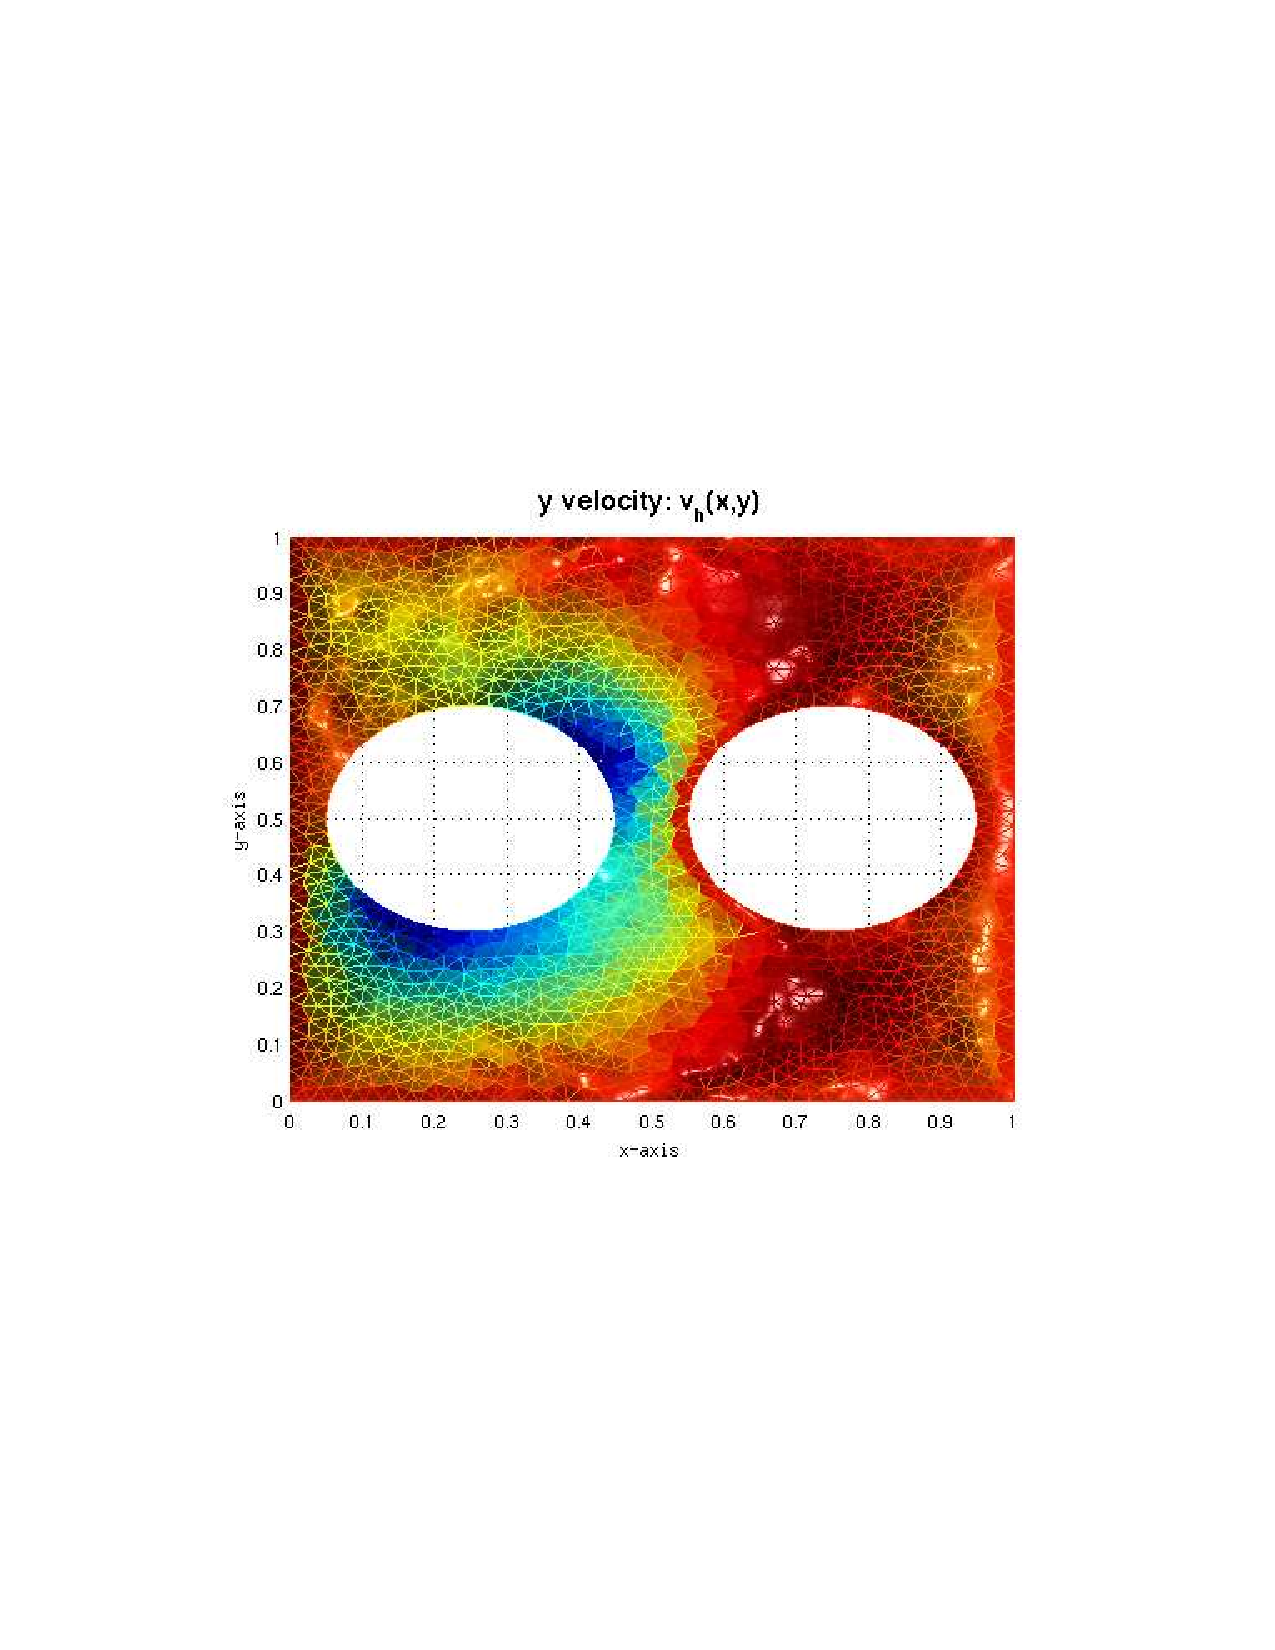
\includegraphics[scale=0.50]{./../files/crazy/v.pdf}
                \caption{$v_h(x,y)$ for $h = 0.025$}
            \end{center}
            \end{figure}

                \section{Conclusions}

                To summarize, I was able to implement a mixed finite element solver
                for the Stokes equation with homogeneous boundary conditions and zero-mean pressure.
                The original intent was to use this to solve the steady-state Navier-Stokes equations
                with Newton's method. Unfortunately, calculating and correctly implementing the Jacobian of the non-linear Navier-Stokes
                system proved too much of a challenge.

                I was able to prove that the error is optimal for the Taylor-Hood $\mathbb{P}_2 - \mathbb{P}_1$ finite element.
                In terms of numerical work, I need to find a closed-form solution to test the actual convergence rates of my implementation
                against the theoretical results.

                \clearpage

                \begin{thebibliography}{9}

                        \bibitem{br}
                        Dietrich Braess,
                        \emph{Finite elements: Theory, fast solvers, and applications in
                        solid mechanics}.
                        Cambridge University Press,
                        Third Edition,
                        2006.

                        \bibitem{vp}
                        Vivette Girault and Pierre-Arnaud Raviart,
                        \emph{Finite Element Methods for Navier-Stokes Equations: Theory and
                        Algorithms}.
                        Springer-Verlag, Germany,
                        1986.

                        \bibitem{j}
                        Claes Johnson,
                        \emph{Numerical Solution to Partial Differential Equations by the
                        Finite Element Method}.
                        Dover, Mineola, New York,
                        2009.

                        \bibitem{nm}
                        Sang Dong Kim, Yong Hun Lee, and Byeong Chun Shin,
                        \emph{Newton's Method for the Navier-Stokes Equations with
                        Finite-Element Initial Guess of Stokes Equation},
                        Computers and Mathematics with Applications 51 (2006),
                        pp. 805 - 816.

                        \bibitem{ds}
                        J.E. Dennis, Jr. and Robert B. Schnabel,
                        \emph{Numerical Methods for Unconstrained Optimization and Nonlinear
                        Equations},
                        Prentice-Hall, Inc, Englewood Cliffs, New Jersy, 1083.

                        \bibitem{c}
                        Philippe G. Ciarlet,
                        \emph{The Finite Element Method for Elliptic Problems},
                        North Holland Publishing Company,
                        Volume 4,
                        1978.

                \end{thebibliography}

                \end{document}

